\section{Experiments} \label{sec:experiments}


\subsection{Baseline Methods} \label{subsec:baseline}

In this section we will go through the experiments performed in order to get
our baseline results. While many different features can be used when performing
\gls{NLP}, we chose the same features, as was used in \cite{US}, since they
span several several of the different linguistic layers. The linguistic layers
are different areas which all serve to describe a certain text. An example this
could be the character level layer, which as the name implies, focuses on the
individual characters used in a specific text. Other examples of this, could
be the sentence layer, that focuses on the sentences of the text, and the meta
layer, that focuses on things such as publishing/delivery date, and file format.
The features available to pick from in this case are:

\begin{itemize}
    \item Word-N-grams,
    \item Character-N-grams,
    \item Word Frequencies (word-1-grams),
    \item \gls{POS}-tag-N-grams, and
    \item Special-Character-N-grams,
\end{itemize}

Where an N-gram describes the combinations of sequential elements of size n. In
the case where that element is characters, and n is 3, the string "hello" would
produce the character-3-grams "hel", "ell" and "llo". This also means that a
feature such as word frequencies can be considered word-1-grams.

\gls{POS} tags, refer to the grammatical class a certain words belongs to, such
as nouns and adjectives. In order to extract these we made use of a POS-tag
extractor, provided by \cite{polyglot}.

For all of these experiments a Danish third party corpus, provided by
\texttt{NLTK}\footnote{\url{http://www.nltk.org/index.html}}, was used as the
basis for all the feature extraction, as was done in \cite{US} as well. This
corpus consists of 22,476 sentences, and 563,358 words.

The actual implementation of both the \gls{SVM} and the Extended Delta method,
very closely resembles the implementation used in \cite{US}. There is however a
very big difference, with the actual application of the delta method. Contrary
to the scenario in \cite{US}, where PAN data was used, there is not an instance
where we only have 1 text per author. As such the original version of the
delta method can be used.\cite{evert2015towards} This is where, when given a
new text $x$ supposedly written by an author $\alpha \in \mathcal{A}$, his
texts $T_\alpha$ are extracted, and so is a set of texts no written by him
$\overline{T}_\alpha$ where $|\overline{T}_\alpha| = |T_\alpha|$. The text,
along with a negative sample text $z$, we know now to be written by $\alpha$ is
given to a \gls{KNN} classifier, which determine if $x \in T_\alpha$ and $z \in
\overline{T}_\alpha$.

\subsubsection{Feature Selection}

The larger part of the experiments performed using the baseline methods, was
centered around parameter tuning. Not only parameter as the K in the extended
delta method, but also the feature supplied to the method. Other methods such
as random forest has a built in filter for bad and noisy feature. This is not
the case for both the \gls{SVM} and extended delta method, who does performs any
kind of quality analysis of the feature they are given, making them susceptible
to the negative influences these features include. It is for this reason that
we chose to select the features for them, rather than just having them use the
entire set available to them.

Contrary to our previous work made in \cite{US}, this process did not
consist of trying out some random selection of features, but rather
a more systematic approach was used.

However, before starting to do that, a feature set had to be created
first. In order for us to find the very best set of features, we wanted
to create a very large initial feature set, so as to increase our search space.
The corpus used had the following quantities of the different features.

\begin{itemize}
    \item Word-2-grams - 188,472
    \item Character-2-grams - 2,178
    \item Word Frequencies - 27,535
    \item \gls{POS}-tag-2-grams - 219
    \item Special-character-2-grams - 524
\end{itemize}

The quantities here are of course very large due to the size of the corpus,
and will continue to rise as N increases. Rather than extracting all
of those feature from our texts, we chose to focus on the N-grams
with highest frequency, as we would reach a point where a specific N-gram
determined to be in the corpus, would be unique that same corpus, making it
irrelevant for new texts, not associated with the corpus.

Using the quantities listed above as inspiration, a feature set of 4950
features was produced, containing

\begin{itemize}
    \item The 500 most frequent words,
    \item The 500 most frequent word-N-grams for $N \in \{2,3,4\}$,
    \item The 300 most frequent character-N-grams for $N \in \{2,...,10\}$,
    \item The 50 most frequent \gls{POS}-tag-N-grams for $N \in \{3,4\}$, and
    \item The 50 most frequent special-character-N-grams for $N \in \{2,3,4\}$.
\end{itemize}

The selection the quantities, bases on the number available in the corpus,
as listed earlier. As the for the N in the N-grams, \cite{aalykke2016} found
out that char-8-grams worked very well in his case, which is why N goes all
the way to 10 in the case of char-N-grams . Looking at the results
from \cite{US}, Word-N-grams mostly stopped occurring in texts when getting
to 4-grams, when looking at the result from \cite{US}. A similar thing
could be seen with the special-character-N-grams, where an increase in N,
would not contribute anything. \gls{POS}-tag-N-grams were a really big burden
computationally, as such a reduction in possible N-values, had to be made.

These features were extracted from the same data-set described earlier in
Section \ref{sec:data}. However it was not beholden to the same exact limits to
character and unique characters. In the case of the upper limit the lack of
memory was not nearly as severe as in the case of our \gls{NN}s. As for the lower
limit, and natural boundary would occur throughout the extraction process.
If a file did not have 500 unique words for example, the extraction
of the 500 most frequent words would cause an error, resulting in that
text being ignored.
The distribution of the texts over authors in this data-set is not
very evenly spread. As such, the random selection of random opposing
authors has a certain amount of bias towards the authors with a large
amount of texts compared to the test.

Having the features, we could start doing our feature selection. This whole
process proved very expensive computationally. Having to check every combination
of 5000 features, simply was not feasible. It was for that reason we opted for a
greedy algorithm instead.

Before starting any kind of feature selection or hyper-parameter tuning,
we split the training data up into training and validation, with a
80/20 respective split. All the work described from this point on,
was done on the 80\% training data set.

The greedy algorithm works as described by \cite{kanDeng}, which is a simple
forward feature selection. Having out previously created feature set, we loop
through each single feature, validating its' accuracy when applied to each
$\alpha \in \mathcal{A}$. As eluded to earlier, this consists of fetching
$T_{\alpha}$ and a set $\overline{T}_{\alpha}$, where $|\overline{T}_\alpha| =
|T_\alpha|$. Using this set of positive and negative cases, we make use k-fold
cross validation to determine the performance of the feature for that author.
This is done for all authors, and when averaged we have the performance of
that single feature. This process is then repeated for all features. The best
performing feature is then added to out candidate set of features. The next
iteration we loop through all the feature again, but we validate against each
feature in combination with the already selected features. This process is
repeated until a set number of features are selected. At this point we determine
at which point we had the best candidate set, and use that hence fourth.

Even this greedy approach proved to be very time consuming. As such, we only did
as described and found the best features, but left out the hyper-parameters C,
and $\gamma$ for the SVM, and K and the distance metric for the extended delta
method. These hyper-parameters were selected through a separate process
which will be described in a later section.

Due to the increased run-time when using leave one out cross validation,
we had to make use of some other model selection approach. Under normal
circumstances, normal X-fold cross validation would work out fine, but a complication
arose when doing this with the extended delta method, which yielded normal
cross validation unfit for that specific classifier.
The reason for this was that there was a scenario where an unlucky split of
folds would cause a lot of error. A generic example of this would be if we
had the 2 class training set consisting of 6 value, evenly split between the
2 classes. In the case where we split those 6 values into 3 folds, there is a
chance that a fold contains two value of the same class, which means that if $K
= 3$ in our case, both of those wont ever be able to classified correctly as
there is only 1 of that class in the training set. As such, stratified K fold
cross validation is used instead, as it uphold the class distribution in its'
folds. While this problem would not plague the SVM classifier, we also opted
the stratified K fold cross, so we would more directly compare the feature selection
of the two models.

For both the \gls{SVM} and Extended Delta method, we ran this algorithm until
350 features were selected. Computation time was still and issue, so we also
limited the computed on dataset to only 5\% of the total number of authors. The
SVM performed its' feature selection using the default RBF kernel, a C with
value 1, and $\gamma = \frac{1}{\text{n\_features}}$. Due to some authors having
below 3 texts, the default K value of \gls{KNN}s K parameter was set to 3 for
the feature selection.

The results of both the SVM and the Extended Delta method feature selection can
be seen in Figure \ref{fig:fs_results}. We got that the best number of selected
feature were 75 for the SVM and 10 for the Extended Delta Method, scoring an
accuracy of 0.675 and 0.666 respectively.

\begin{figure}
    \centering
    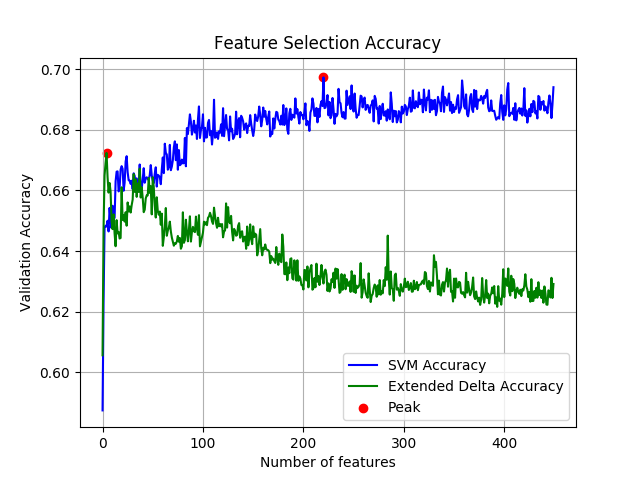
\includegraphics[scale=0.8]{./pictures/experiments/FeatureSelect.png}
    \caption{The process of the greedy feature selection of the SVM and the Extended Delta Method}
    \label{fig:fs_results}
\end{figure}


\subsubsection{Hyper Parameter Selection}

As mentioned in the previous section, due to computational time, we were unable
to do the hyper parameter selection parallel with the feature selection.
For that reason we chose to split it up, selecting our features first, and the
fine tuning our parameters based on those selected features.

This means that our implementation very closely mimics the one used in the
previous example. On both cases we start out with two lists of possible hyper
parameter values:

\begin{align}
    \text{SVM} &:
    \begin{array}{lr}
        C=\{10^{-16}, 10^{-14}, 10^{-12}, 10^{-10}, 10^{-8}, 10^{-6}, 10^{-4}, 10^{-2}\} \\
        \gamma=\{10^{-3}, 10^{-1}, 10^{1}, 10^{3}, 10^{5}, 10^7\}
    \end{array} \\
    \text{Extended Delta} &:
    \begin{array}{lr}
        p=\{1,2,3,4,5\}\\
        K=\{1,3,5,7,9,11,13,15\}
    \end{array}
\end{align}

The one parameter yet to be explained i $p$, which refers to the p in the
minkowski distance,

\begin{equation}
    D(X,Y) = \left(\sum_{i = 1}^n |x_i - y_i|^p\right)^{1/p},
\end{equation}

where $p=1$ and $p=2$ is the manhattan and eucledian distance respectively.

We perform a grid search over all these parameters. For each variation of the
hyper parameters we average the performance of the method over all unique
authors in the training set, in a manner very similar to the feature selection.
We make use of the same 3-fold stratified cross validation, and arrange each
authors with set of opposing set of text, amounting to the same number he has
written himself. The accuracy of each parameter configuration can be seen
in Table \ref{sec:ed_feat} for \gls{KNN}, and Table \ref{sec:svm_feat} for
\gls{SVM}.

\begin{table}[h]
    \centering
    \caption{The results from performing a grid search of the p and K parameter
        of the \gls{KNN} algorithm}
    \label{table:KNN}
    \begin{tabular}{|c|ccccc|}
        \hline
        \backslashbox{$K$}{$p$} & 1 & 2 & 3 & 4 & 5 \\\hline
        1 & \textbf{0.647} & 0.622 & 0.608 & 0.593 & 0.591 \\
        3 & 0.646 & 0.617 & 0.598 & 0.586 & 0.580 \\
        5 & 0.640 & 0.603 & 0.586 & 0.572 & 0.565 \\
        7 & 0.627 & 0.593 & 0.571 & 0.561 & 0.554 \\
        9 & 0.620 & 0.581 & 0.562 & 0.550 & 0.543 \\
        11 & 0.608 & 0.566 & 0.549 & 0.541 & 0.535 \\
        13 & 0.598 & 0.558 & 0.539 & 0.533 & 0.529 \\
        15 & 0.590 & 0.546 & 0.536 & 0.527 & 0.522 \\\hline
    \end{tabular}
\end{table}

\begin{table}[h]
    \centering
    \caption{The results from performing a grid search for C and gamma, of the
        \gls{SVM} algorithm}
    \label{table:SVM}
    \begin{tabular}{|c|cccccc|}
        \hline
        \backslashbox{$C$}{gamma} & $10^{-3}$ & $10^{-1}$ & $10^{1}$ & $10^{3}$ & $10^{5}$ & $10^{7}$ \\\hline
        $10^{-16}$ & 0.592     & 0.592     & 0.592    & 0.593    & 0.648          & 0.621    \\
        $10^{-14}$ & 0.592     & 0.592     & 0.592    & 0.630    & \textbf{0.679} & 0.601    \\
        $10^{-12}$ & 0.592     & 0.592     & 0.628    & 0.631    & 0.678          & 0.591    \\
        $10^{-10}$ & 0.592     & 0.629     & 0.629    & 0.631    & 0.678          & 0.585    \\
        $10^{-8}$  & 0.589     & 0.629     & 0.629    & 0.631    & 0.678          & 0.581    \\
        $10^{-6}$  & 0.587     & 0.629     & 0.629    & 0.631    & 0.678          & 0.576    \\
        $10^{-4}$  & 0.587     & 0.629     & 0.629    & 0.631    & 0.678          & 0.573    \\
        $10^{-2}$  & 0.587     & 0.629     & 0.629    & 0.631    & 0.678          & 0.568   \\\hline
    \end{tabular}
\end{table}

It is at this point we grab the 20\% of we set aside at the start of our
experimentation. While applying these finely tuned methods to a validation set
wont change anything in terms of the parameters we have selected, it will give
us the ability to gauge the accuracy of our methods when applied to a new, never
before seen, test-set.

\begin{center}
\begin{verbatim}
Extended Delta Validation Accuracy: 0.602
SVM Validation Accuracy:  0.684
\end{verbatim}
\end{center}


\subsection{Deep Learning}

In the prediction system from Definition \ref{def:prediction_system} we needed
a function $f$ that takes two texts and returns the probability that those
texts are written by the same author. As described earlier Siamese Neural
Networks are well suited for comparing objects. In this Section we describe
the experiments we performed with different networks architectures and we
will present three different networks. The three networks are \gls{conv-char-NN}
in Section \ref{subsubsec:conv_char_nn}, \gls{conv-char-word-NN} in Section
\ref{subsubsec:conv_char_word_nn}, and \gls{rec-sent-NN} in Section
\ref{subsubsec:rec_sent_nn}.

The data we trained our networks on is described in Section \ref{sec:data}. We
trained the networks on the G dataset that contains 3000 authors. We used early
stopping based on a validation dataset H that contains 500 authors. Through
experimentation we found that the validation dataset had to contain completely
different authors than the training dataset. In the beginning of our project we
had a validation set that contained different problem instances (two texts to
compare) from the training set but contained some of the same authors. That lead
to the validation set not being a very good estimate of the networks performance
on different authors than the ones seen during training. The networks were
therefore overfitting on the specific authors and we could not see that in the
validation datasets accuracy. All accuracy graphs shown in this Section are
based on a validation dataset with 500 completely unseen authors.

The general structure of our networks will be that they take two texts as input.
The texts are first embedded into a format that can be used by the network.
Then the texts are transformed into two sets of features representing the text
via a weight sharing network. Then the text representation will be combined
in some way and a dense network will take the combined representations and
decide whether or not the texts are written by the same author. We call the
different parts of the network \textit{Embedding}, \textit{Feature Extraction},
\textit{Combining} and \textit{Decision}.

When we show graphs of the networks we have produced we use specific names for
different layers in the networks. A glossary of the layer names and paramters of
the layers are shown in Table \ref{tab:glossary}.

\begin{landscape}
    \begin{table}
        \centering
        \caption{Glossary used when performing experiments, and creating their
            associated models.\cite{chollet2015keras}}
        \label{tab:glossary}
        \begin{tabular}{|L{3cm}|L{9cm}|L{11cm}|}
            \hline
            \multicolumn{1}{|c|}{\textbf{Layer}}                               &
            \multicolumn{1}{|c|}{\textbf{Description}}                         &
            \multicolumn{1}{|c|}{\textbf{Actively Used Parameters}}           \\
            \hline

            Input                                                              &
            Serves as the entrypoint of the network, by receiving a set of
            texts and feeding it trough the network.                           &
            \begin{minipage}[t]{\linewidth}
            \begin{compactdesc}
                \item[Shape] The dimensions of each sample give to the input.
            \end{compactdesc}
            \end{minipage}                                                    \\
            \hline

            Embedding                                                          &
            Taking in an encoded sample, it produces a dense vector
            representation for each different. More details can be found in
            Section \ref{subsubsec:layers}.                                    &
            \begin{minipage}[t]{\linewidth}
            \begin{compactdesc}
                \item[Input Dim] Size of vocabulary.
                \item[Output Dim] Size of vector used to represent embedding.
            \end{compactdesc}
            \end{minipage}                                                    \\
            \hline

            Convolutional                                                      &
            Applies convolution to the data it recieves according to the
            decription, found in Section \ref{subsubsec:layers}.               &
            \begin{minipage}[t]{\linewidth}
            \begin{compactdesc}
                \item[Filters] Dimensionality of the output, ie. number of
                    filter from the convolution.
                \item[Kernel Size] Integer or list describing size of
                    convolution window.
                \item[Strides] Stride length of the convolutional window.
                \item[Activation] The activation function to be applied after
                    the convolution.
            \end{compactdesc}
            \end{minipage}                                                    \\
            \hline

            Global Max Pooling                                                 &
            Extracts the maximum value from each of the provided data          &
            No parameters.                                                    \\
            \hline

            Concatenation                                                      &
            As the name suggests, this layers simply concatenates the data it
            receives from different layers                                     &
            No parameters.                                                    \\
            \hline

            Merge                                                              &
            Merges its inputs, using a specified function to generate a single
            output.                                                            &
            \begin{minipage}[t]{\linewidth}
            \begin{compactdesc}
                \item[Function] The function used to merge the recieved data.
            \end{compactdesc}
            \end{minipage}                                                    \\
            \hline

            Dense                                                              &
            A simple fully connected layer, taking in data and applying the
            function described in Section \ref{sec:neurons}.                   &
            \begin{minipage}[t]{\linewidth}
            \begin{compactdesc}
                \item[Units] Number of neurons in in the layer.
                \item[Activation] The activation function to be applied.
            \end{compactdesc}
            \end{minipage}                                                    \\
            \hline

            Dropout                                                            &
            Drops a fraction it receives, with the goal of preventing
            overfitting.                                                       &
            \begin{minipage}[t]{\linewidth}
            \begin{compactdesc}
                \item[Rate] The fraction of data it receives dropped.
            \end{compactdesc}
            \end{minipage}                                                    \\
            \hline

            Lambda                                                             &
            Applies a specified function to the input it receives              &
            \begin{minipage}[t]{\linewidth}
            \begin{compactdesc}
                \item[Function] The function applied.
            \end{compactdesc}
            \end{minipage}                                                    \\
            \hline

            Reshape                                                            &
            Reshapes the data it receives.                                     &
            \begin{minipage}[t]{\linewidth}
            \begin{compactdesc}
                \item[Dim] Dimensionality to reshape to.
            \end{compactdesc}
            \end{minipage}                                                    \\
            \hline

            LSTM                                                               &
            A Long Short-Term Memory layer, which works according to the
            description in Section \ref{subsubsec:layers} is applied to the
            given data.                                                        &
            \begin{minipage}[t]{\linewidth}
            \begin{compactdesc}
                \item[Unit] Number of neurons in the layer.
            \end{compactdesc}
            \end{minipage}                                                    \\
            \hline
        \end{tabular}
    \end{table}
\end{landscape}


\subsubsection{\glsdesc{conv-char-NN}}
\label{subsubsec:conv_char_nn}

The idea behind network \gls{conv-char-NN} is that we wanted to use convolutions
to look for n-grams in texts. Traditional authorship verification/attribution
is based on carefully engineered n-grams that are compared between two texts
\cite{stamatos2009}. Instead of choosing the n-grams ourselves we wanted the
network to learn which features are important for the authorship verification
task. The features are learned through convolutions. The convolutions look
at some number of characters at a time and gives a single output for those
characters. Assume for example that the network has learned that the character
sequence "ould " is important for deciding the author of a text. Then we
expect the network to react strongly to character sequences that looks
like "ould ". We have illustrated such a convolutional filter in Figure
\ref{fig:convolution_text_example}.

\begin{figure}
    \centering
    \textbf{Convolutions for Text Feature Extraction}\par\medskip
    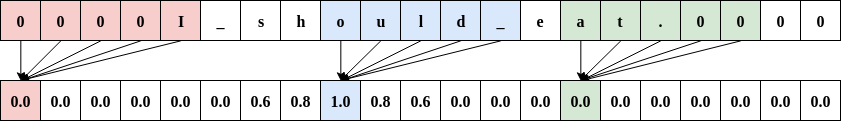
\includegraphics[width=\textwidth]{./pictures/experiments/convolution_example.png}
    \caption{Illustration of character level convolutions using a filter that
        looks for the character sequence "ould ". Notice that high values are
        produced when the characters the filter looks at match the characters it
        is looking for and low values are produced otherwise. We have
        illustrated 3 different filter locations but the filter is similarly
        placed in all possible locations. We have padded the text with zeros to
        get the same size output as input.}
    \label{fig:convolution_text_example}
\end{figure}

\begin{description}

    \item[Embedding:]

        The embedding takes as input a sequence of integers. Each different
        integer is a compact one-hot encoding of each character. The one-hot
        encoded character stream is embedded in a five dimensional space. The
        hope is that the layer will learn that similar characters should be
        placed close to each other in the output space and dissimilar characters
        should be placed far apart. The same embedding is performed on both of
        the input texts and the layer is therefore part of the Siamese part of
        the network.

    \item[Feature Extraction:]

        Features are extracted from the two texts via a layer of convolutions
        with different sizes. We use both convolutions with a window size of
        8 and convolutions with a window size of 4. We use 700 of size 8 and
        500 of size 4. We used a window size of 8 since \cite{aalykke2016}
        found that n-grams of size 8 worked the best for Danish texts and we
        also added 4 so the network could look at smaller n-grams as well.
        We used a stride of 1 such that each convolutional filter could
        observe all parts of the texts and give an output for each one. The
        convolutional part of the network also shares weights such that the
        same features are extracted from both the input texts. We use the
        \gls{ReLu} activation function for the reasons described in Section
        \ref{subsubsec:activation_functions}.

        After the convolutional layer we added a global max pooling layer. The
        layer takes the maximum output of each convolutional filter. We do that
        as the output size of the convolutional layer depends on the length of
        the input text. The output of the max pooling layer is $700 + 500 =
        1200$ numbers, one for each convolutional filter. That means that the
        network learns to extract 1200 different features from each text.

    \item[Combining:]

        The features of the texts are combined using the absolute difference
        function. As described each text is represented as a vector of 1200
        features and to combine them we subtract them from each other and take
        the elemtwise absolute difference.

    \item[Decision:]

        The decision part of the network consists of 4 dense layers each with
        500 neurons, a dropout layer and an output layer. The 4 dense layers
        also use the \gls{ReLu} activation function. The dropout layer is added
        just before the output layer and performs 30\% dropout to try to combat
        overfitting. The actual prediction is performed in the output layer. The
        output layer use the softmax function to return a probability
        distribution over the two possibilities that the texts are written by
        the same author and that they are written by different authors.

\end{description}

We have shown an illustration of the network in Figure \ref{fig:conv-char-NN}.
In the Figure we have illustrated the Siamese part of the network as a blue box.
The 4 phases of the network is not illustrated in the Figure but it should be
possible to find them by reading the description above. We trained the network
on the dataset described in the Section \ref{sec:data} and in the beginning
of this Section. We used the \gls{Adam} optimizer during the training of the
network. We used a learning rate of $\eta = 0.0005$, half of what was suggested
by \cite{DBLP:journals/corr/KingmaB14}. We did that as we had problems with
neurons dying during the training of the network otherwise. Other than the
learning rate we used the parameters suggested in the article. That is, the
remembering rates were set to $\gamma_1 = 0.9$ and $\gamma_2 = 0.999$. As the
error function we used the Categorical Crossentropy function described in
Section TODO. When we trained the network we were able to obtain a validation
accuracy of 0.71773 in epoch 6. The training accuracy continued rising but we
used early stopping since the validation accuracy had stopped improving. We have
shown a graph of the training and validation accuracies during training in
Figure \ref{fig:conv-char-NN-accuracies}. During the training we used minibatch
learning with a minibatch size of 8. We used a size of 8 as that was the largest
batch size that could fit in the GPUs memory. During the training we padded all
texts with zeros such that all texts in each batch had the same length. We did
that as it is required by Keras. We have shown the training and validation
accuracies during training in Figure \ref{fig:conv-char-NN-accuracies}.

\begin{figure}
    \centering
    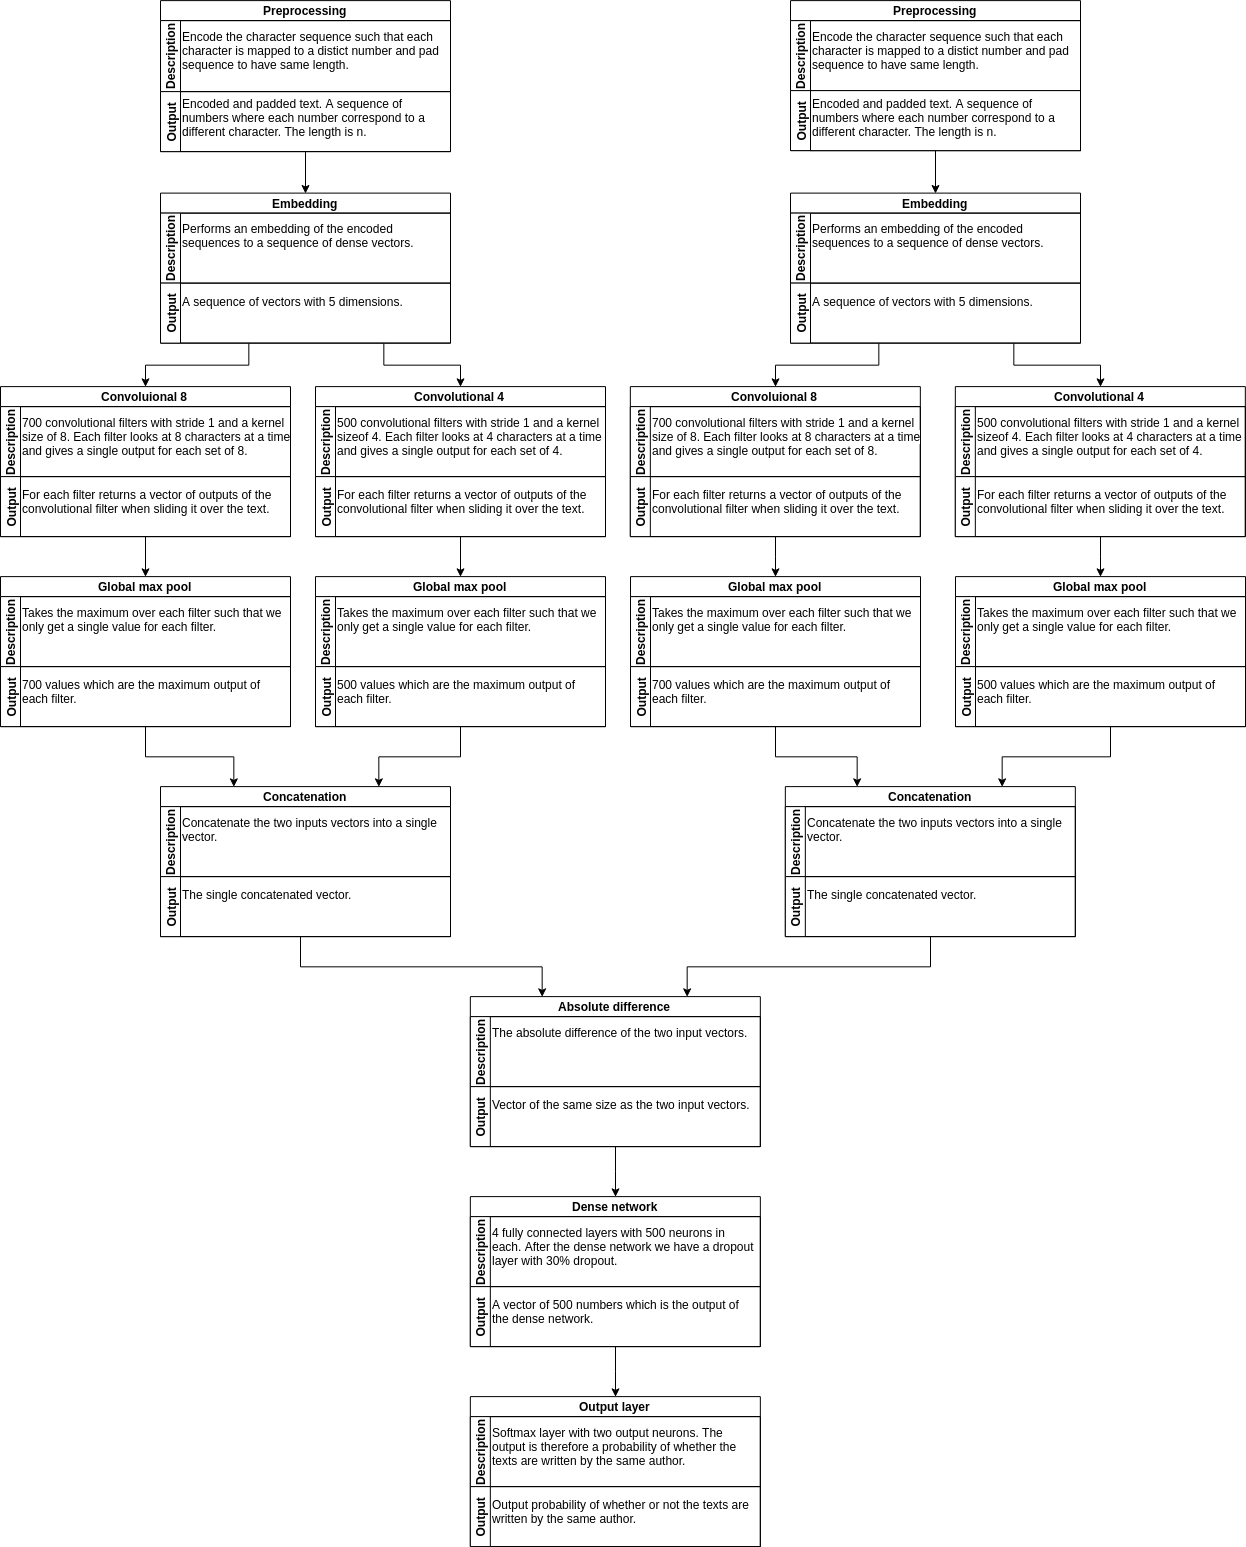
\includegraphics[width=\textwidth]{./pictures/experiments/network3.png}
    \caption{The structure of network \gls{conv-char-NN}. Weights are
        shared by the embedding layers and the convolutional layers as shown by
        the blue box. The input to the network is at the top and the output is
        at the bottom. Information flows downwards through the layers. The final
        softmax layer produces a probability distribution over the two
        possibilities that the texts are either written by the same author or
        not.}
    \label{fig:conv-char-NN}
\end{figure}

\begin{figure}
    \centering
    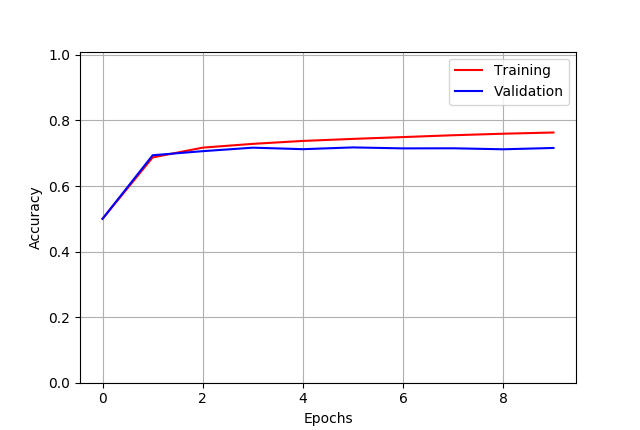
\includegraphics[width=\textwidth]{./pictures/experiments/conv-char-NN-training-accuracy.png}
    \caption{The training and validation accuracy of \gls{conv-char-NN} during
        training. Each epoch contains several thousand minibatches which is why
        the training and validation accuracies rises so much in the first
        epoch.}
    \label{fig:conv-char-NN-accuracies}
\end{figure}

To arrive at the network architecture described above we experimented with
several similar architectures. We started with a network that used,

\begin{description}

    \item[Embedding:]

        Same as described above.

    \item[Feature Extraction:]

        1000 convolutional filters of size 10.

    \item[Combining:]

        Instead of the absolute difference we used a concatenation of the
        feature vectors extracted from the two texts. If we let the extracted
        features of the first text be $T_{1,i}$ and the extracted features of
        the second text be $T_{2,i}$ then $T_{1,0}$ and $T_{2,0}$ correspond to
        the same feature extracted from the two texts. The concatenation
        combining function would then compute,

        \begin{equation}
            combine(T_1, T_2) \rightarrow \left(
                T_{1,0}, T_{1,1}, \dots, T_{1,n}, T_{2,0}, T_{2,1}, \dots, T_{2,n}
            \right)^T.
        \end{equation}

    \item[Decision:]

        We used a small dense network with only a single hidden layer of 500
        neurons. The output layer was similar to the one described above. 

\end{description}

The network gave promising results which is why we continued working with it but
it quickly overfitted on the training data so we added some dropout. Like in
the network presented above we added the dropout layer just before the output
layer and used 30\% dropout. That regularization allowed the training accuracy
and validation accuracy to follow each other for more epochs making the final
validation accuracy better.

We changed the combining function from a concatenation to a absolute difference
since the network would then not have to learn which features belonged to other
features. The new combination function is computed as,

\begin{equation}
    combine(T_1, T_2) \rightarrow \left(
        (|T_{1,0} - T_{2,0}|), (|T_{1,1} - T_{2,1}|), \dots, (|T_{1,n} - T_{2,n}|)
    \right)^T.
\end{equation}

We also tried other combining functions such as the cosine difference but we
didn't get any better results. After that change we changed the convolutional
filters from using 1000 filters of size 10 to using 500 filters of size 8 and
500 of size 4. We used those window sizes for the reasons described above. At
the same time we added more dense layers to the model. We again observed the
validation accuracy increasing further.

%As described our first network took as input two sequences of characters. Each
%character was then one-hot encoded and as described in Section \ref{sec:data} we
%ignored character with a frequency of less than $10^{-5}$. In the
%\textit{Embedding} part of the network we embedded the characters into a 5
%dimensional space. The embeddings are learnable and the hope is that similar
%characters will end up in similar places in the output space.

%In the \textit{Feature Extraction} part of the network we applied 1000
%convolutional filters of size 10 to each of the texts. We used stride 1
%such that each filter was placed in all possible positions. We did not
%use padding in the convolutional layer so the output will be slightly
%smaller than the input. As the activation function in the convolutional
%layer we used the \gls{ReLu} function for the reasons described in Section
%\ref{subsubsec:activation_functions}. After the convolutional layer we applied a
%global max pooling layer. The global max pooling layer will output the maximum
%activation for each filter in the convolutional layer. We do so for both of the
%texts so afterwards we will have two vectors containing 1000 numbers each. The
%first vector represent the maximum activation of the 1000 filters on the first
%text and the second vector represents the maximum activation of the 1000 filters
%on the second text. These 1000 numbers are seen as the extracted features of the
%texts and they will represent the text in the following layers.

%In the \textit{Combining} part of the network we concatenate the representations
%of the two texts to obtain a single vector of size 2000.

%Lastly the \textit{Decision} network takes the combined vectors and applies a
%fully connected network to it. The fully connected network consist of a layer
%with 500 neurons using the \gls{ReLu} activation function and a layer of two
%neurons using the softmax activation function. The idea is that the hidden dense
%layer will compare the vector representations and that the output layer will
%output a probability distribution. The probability distribution represents the
%probability that the texts are written by the same author.

%As the optimization function we use the \gls{Adam} optimizer. We used the
%default parameters of $\eta = 0.001$, $\gamma_1 = 0.9$ and $\gamma_2=0.999$.
%As the loss function we used the categorical crossentropy function.

%When we trained the network it quickly overfitted on the training dataset but
%otherwise it seemed to work fine. We therefore wanted to try to extend the
%network and add some dropout.


\subsubsection{\glsdesc{conv-char-word-NN}}
\label{subsubsec:conv_char_word_nn}

%\subsubsection{Siamese Neural Network - Iteration 1}

%The network we used to try and solve the problem is shown in Figure
%\ref{fig:network_1}. The Siamese part of the network is the Convolutional
%Layer. We used 1000 filters of size 10. That means that 1000 different features
%are supposed to be learned by the network and each feature can use a local
%context of 10 characters to extract a feature. After the convolution we have a
%max-over-time pooling layer. The layer takes the maximum value of each feature
%such that we have 1000 features from each text. We then have a normal dense
%neural network on top of that which are given the features of both texts. The
%dense network is then supposed to learn how to compare the features from the two
%texts. We have 1 dense hidden layer each with 500 neurons. At the end we have
%a output layer with two outputs. The activation function for all layers except
%the last one is the rectified linear unit and the activation function of the
%last layer is the softmax function. The output of the network is a probability
%distribution over the two classes.

%The input to the network first goes through an embedding layer. The embedding
%layer transforms integers into dense vectors of floating point numbers. The
%embedding layer functions as a lookup table such that each integer is mapped
%to the same dense vector. The embedding is trainable meaning that better
%embeddings will be learned while the network is training.

%\begin{figure}[htb]
    %\centering
    %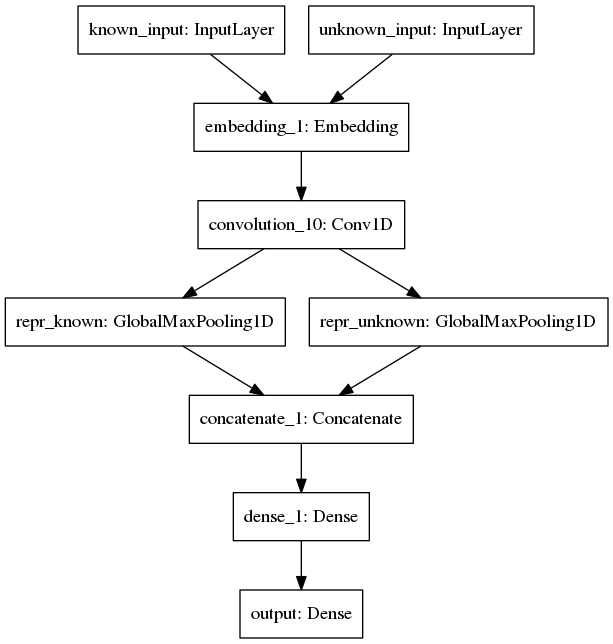
\includegraphics[width=0.6\textwidth]{./pictures/experiments/network1.png}
    %\caption{Illustrate the structure of our first Siamese Neural Network
        %Architecture.}
    %\label{fig:network_1}
%\end{figure}

%The network obtained a validation accuracy of 0.68684. We have shown both the
%training and validation accuracies in the different epochs in Figure
%\ref{fig:network1_accuracies}. In that plot we can see that the network very
%quickly overfits the training data and no longer learns anything general.

%\begin{figure}[htb]
    %\centering
    %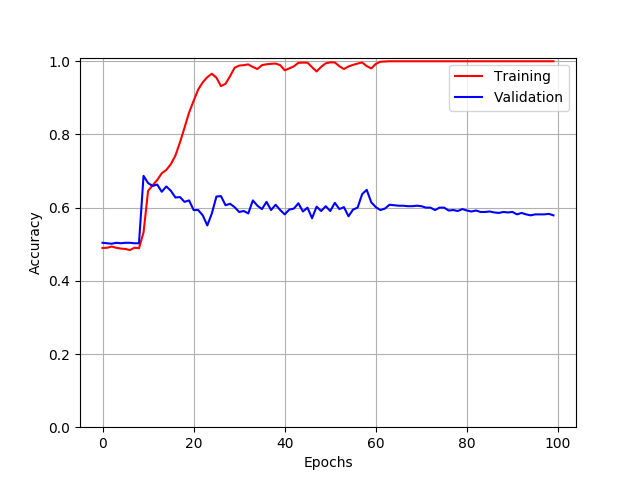
\includegraphics[width=0.5\textwidth]{./pictures/experiments/network_1_accuracies.png}
    %\caption{Training and validation accuracies for the iteration 1 network in
        %the different epochs of the networks execution.}
    %\label{fig:network1_accuracies}
%\end{figure}


%\subsubsection{Siamese Neural Network - Iteration 2}

%In our last network we observed that the network after a few number of epochs
%overfitted on the training dataset. The validation accuracy quickly began
%stalling as the training accuracy went to 100\%. We therefore focused our second
%network architecture on limiting overfitting. We added a dropout layer before
%the output layer.

%In iteration 1 the function we used to merge features from the known and unknown
%text together were a concatenation. If we let the extracted features of the
%known text be $K_i$ and the extracted features of the unknown text be $U_i$ then
%$K_0$ and $U_0$ correspond to the same feature extracted from the two texts. The
%concatenation merge function would then produce,

%\begin{equation} merge(K, U) \rightarrow \left(
        %K_0, K_1, \dots, K_n, U_0, U_1, \dots, U_n
    %\right)^T.
%\end{equation}

%That means that the neural network would have to figure out by itself that input
%$0$ were related in particular to input $n + 1$. To save the network that task
%we also replaced the merging function to the absolute difference of the feature
%vectors. That means that our merge function became,

%\begin{equation}
    %merge(K, U) \rightarrow \left(
        %(|K_0 - U_0|), (|K_1 - U_1|), \dots, (|K_n - U_n|)
    %\right)^T.
%\end{equation}

%So the network no longer has to learn arbitrary indexes. Instead it can learn
%which features is important for authorship verification and learn thresholds for
%when each feature is important. With the new merging we will have a large number
%whenever the two features are far apart and a small number whenever they are
%close to each other.

%We changed the convolutional filters we used from 1000 convolutional filters of
%size 10 to 500 convolutional filters of size 4 and 500 convolutional filters of
%size 8. The idea was that the filters could learn different features where some
%of the features would consist of a large number of characters and other of the
%features would consist of a small number of characters. The architecture of our
%network from iteration 2 is shown in Figure \ref{fig:network_2}.

%\begin{figure}
    %\centering
    %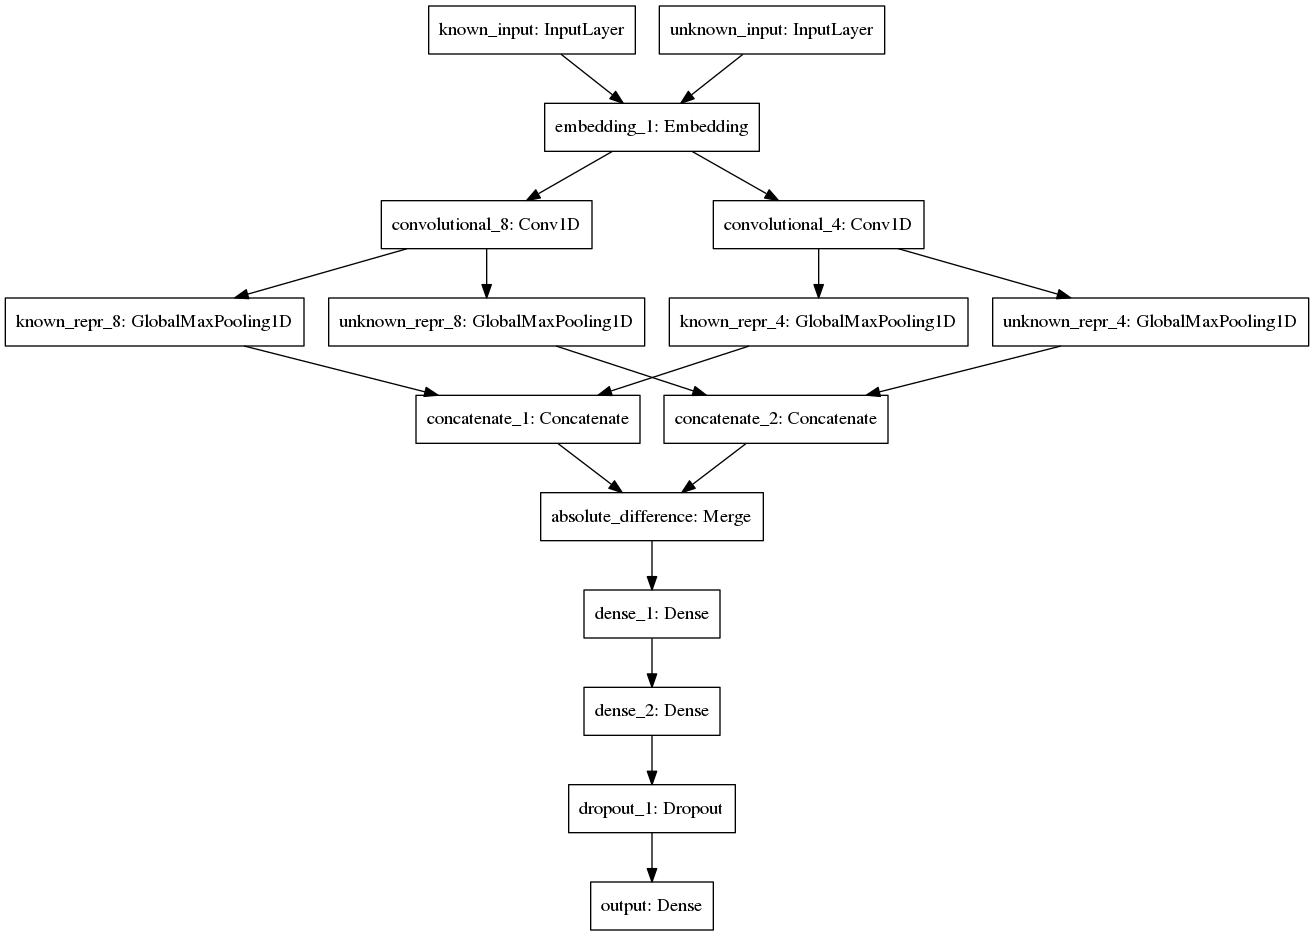
\includegraphics[width=\textwidth]{./pictures/experiments/network2.png}
    %\caption{Illustrate the structure of our second Siamese Neural Network
        %Architecture.}
    %\label{fig:network_2}
%\end{figure}

%We also added more dense layers to the model. A plot of the
%training and validation accuracies per epoch can be seen in Figure
%\ref{fig:network2_accuracies}.

%\begin{figure}
    %\centering
    %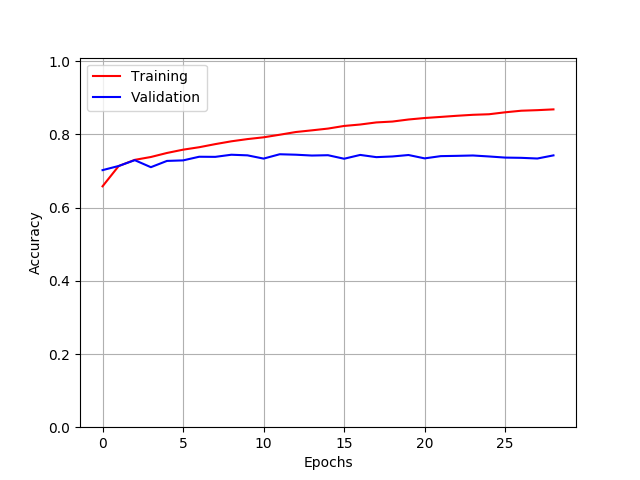
\includegraphics[width=0.5\textwidth]{./pictures/experiments/network_2_accuracies.png}
    %\caption{Shows the training and validation accuracies on the second
        %network.}
    %\label{fig:network2_accuracies}
%\end{figure}

%The maximum validation accuracy obtained were 0.74464 in epoch 12.


%\subsubsection{Siamese Neural Network - Iteration 3}

%In iteration 2 we observed that the network seemed to learn everything in the
%first epoch and did not improve much after that. We also observed that the
%accuracy improved compared to the first network. We therefore wanted to try a
%larger network which would be able to hopefully learn more and obtain a higher
%accuracy than our first two networks.

%We both tried adding more convolutions and adding more dense layers. Our third
%network use 700 convolutions of size 8 (currently drawn confusingly) and 500
%convolutions of size 4. The network then contains 4 dense layers all with 500
%hidden neurons with \gls{ReLu} activation function. Then a dropout layer with
%30\% dropout and finally the output layer with 2 neurons and a softmax
%activation function. The function we use to combine the features from the two
%texts are still the absolute difference as that seemed to work fine for the
%previous network. We have shown the structure of the third network in Figure
%\ref{fig:network3}.

%\begin{figure}
    %\centering
    %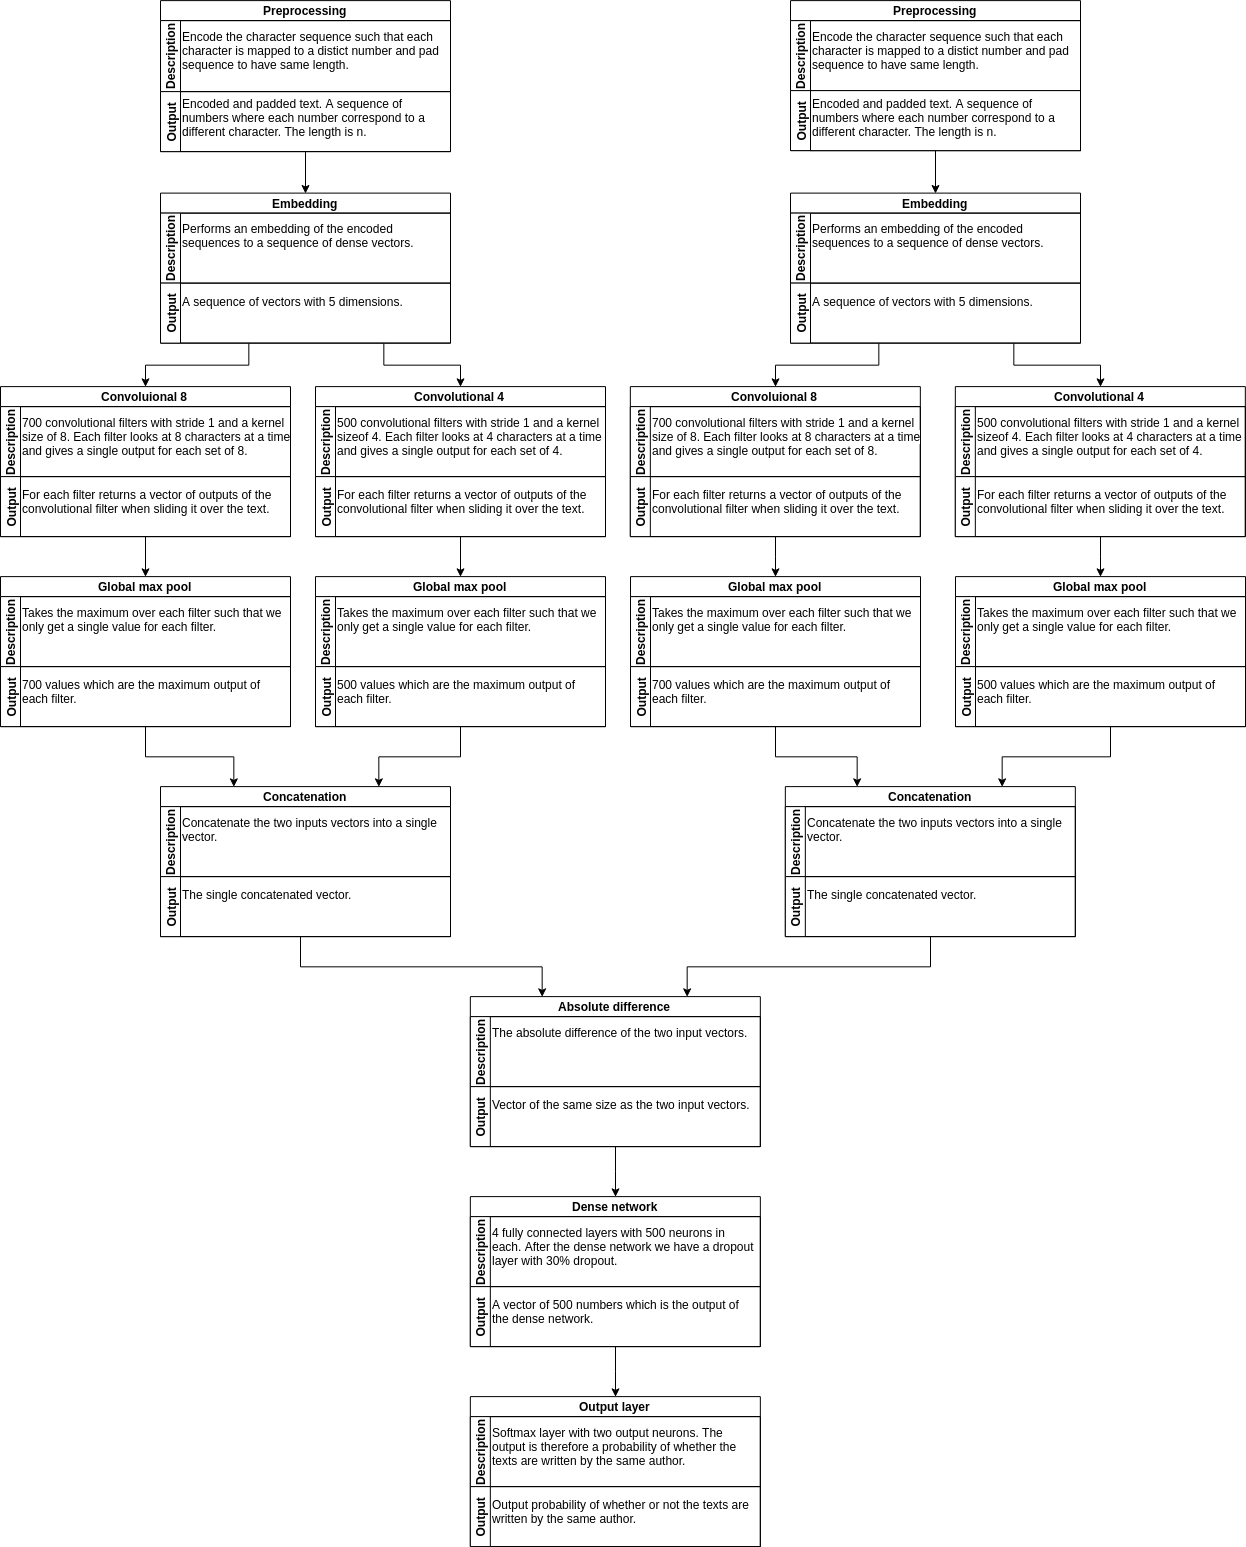
\includegraphics[width=\textwidth]{./pictures/experiments/network3.png}
    %\caption{Illustrate the structure of our third Siamese Neural Network.
        %Weights are shared by the embedding layers and the convolutional
        %layers.}
    %\label{fig:network3}
%\end{figure}

%Our third network were able to obtain an accuracy of 0.83612. We have shown the
%training and validation accuracies in Figure \ref{fig:network_3_accuracies}. We
%can see that the network quickly improve to about 80\% accuracy and after that
%not much happens.

%\begin{figure}
    %\centering
    %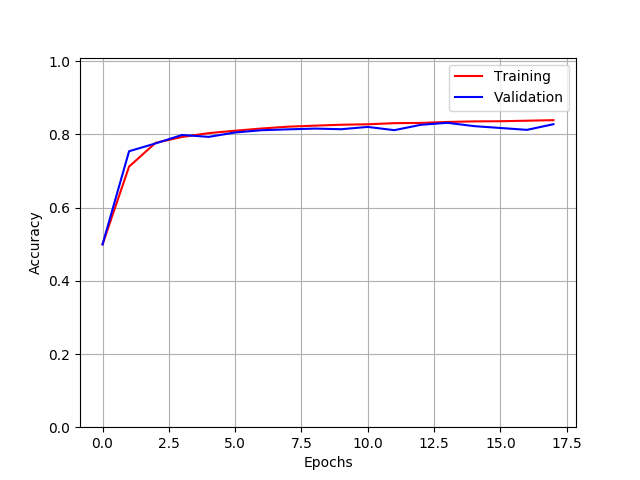
\includegraphics[width=0.5\textwidth]{./pictures/experiments/network_3_accuracies.png}
    %\caption{Shows the training and validation accuracies over the epochs of
        %training on the third network.}
    %\label{fig:network_3_accuracies}
%\end{figure}

%To get an idea of which features the network were looking at we looked at the
%output of the convolutional layers. After the convolutional layers we have a
%max-over-time pool so we know that higher values are important. We could then
%take a text, feed it to the network, find the index of the maximum output of
%the convolutional layers and then show the text snipped (char-N-gram) that
%produced that high value. We then did that for all the texts in the dataset. The
%first filter in the network for example yielded many short strings ending with 3
%newlines. Some examples of these are,

%\begin{lstlisting}[gobble=4]
    %'adsen\n\n\n'
    %'ndsen\n\n\n'
    %'umeer\n\n\n'
    %'endte\n\n\n'
    %'ingen\n\n\n'
    %'ehren\n\n\n'
    %'elsen\n\n\n'
    %'ommer\n\n\n'
    %'Ruter\n\n\n'
    %'ummer\n\n\n'
    %'ersen\n\n\n'
    %'ansen\n\n\n'
    %'heden\n\n\n'
    %'ensen\n\n\n'
    %'arsen\n\n\n'
    %'orten\n\n\n'
    %'ulsen\n\n\n'
    %'orgen\n\n\n'
%\end{lstlisting}

%Many of those short string looks like the ending of common Danish
%names followed by three newlines. Here are some examples of the
%names taken from a list of the 100 most frequent surnames in Denmark
%\footnote{http://www.mydanishroots.com/surnames-meaning-and-origin/the-100-most-
%common-surnames-in-denmark.html},

%\begin{description}
    %\item[adsen:] Madsen.
    %\item[ndsen:] Svendsen, Frandsen.
    %\item[elsen:] Nielsen, Mikkelsen.
    %\item[ersen:] Pedersen, Andersen, Petersen, Iversen, Jespersen.
    %\item[ansen:] Hansen, Christiansen, Johansen, Kristiansen.
    %\item[ensen:] Jensen, Christensen, S\o rensen, J\o rgensen, Kristensen,
        %Mortensen, Mogensen.
    %\item[arsen:] Larsen.
    %\item[ulsen:] Poulsen.
%\end{description}

%The network therefore seems to have learned that a name followed by whitespace
%are an important feature when determining the authorship of a text. Clearly when
%a student buy an assignment from a ghost writer the text will contain the
%students own name. Therefore these features are counter productive since the
%network learns that as a result of how we have created the training dataset
%where each text has the correct authors name in it.


%\subsubsection{Siamese Neural Network - Iteration 4}

%In this iteration we trained the third network again but now using a dataset
%where names were substituted by empty strings. We wanted to see how well the
%network would perform when it was not able to use peoples names as a feature.
%A graph of the training and validation accuracies can be seen in Figure
%\ref{fig:network_4_accuracies}. The best validation result we found was in epoch
%22 with an accuracy of 0.79843. That means that we lost about 4\% accuracy now
%that we can no longer look at peoples names.

%\begin{figure}
    %\centering
    %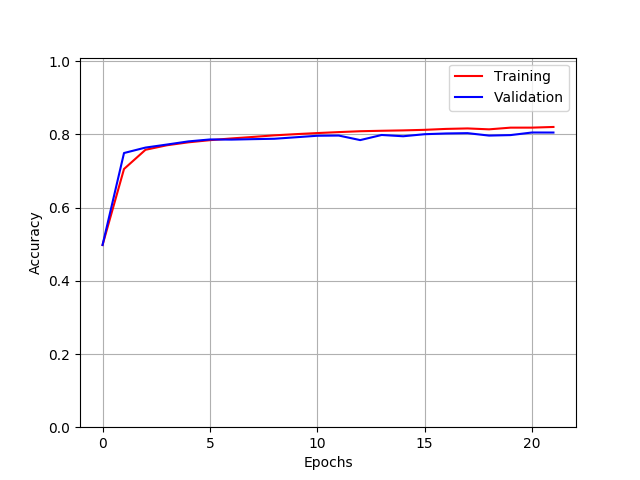
\includegraphics[width=0.5\textwidth]{./pictures/experiments/network_4_accuracies.png}
    %\caption{Shows the training and validation accuracies over the epochs of
        %training on the fourth iteration of the network.}
    %\label{fig:network_4_accuracies}
%\end{figure}

%We wanted to verify whether or not the network still looked at the names of the
%authors. It is not possible for us to look at all 1200 filters but we looked
%at a couple and did not find any that looked like they were looking at names.
%However we did find that the network now seems to be looking at which class
%the student is in. The classes in Danish schools are typically written as 1.p,
%1.q, 2.p, 2,q, etc. and we found that one of the convolutional 4 filters were
%looking at character sequences such as those. We have generated a couple of
%tables that shows what the network is now looking at. We generated the tables by
%taking the first 50 texts from the dataset and extracting the maximum value of a
%particular filter from each text. That gives a single string of the convolution
%size from each text and a number which is higher the more important that string
%is. We then sorted the extractions by the importance score. The result of a
%couple of the filters are shown in Figures \ref{fig:features_convolution_8_1},
%\ref{fig:features_convolution_8_5}, \ref{fig:features_convolution_8_100} and
%\ref{fig:features_convolution_4_100}. The first figure looks at whether or not
%authors use the phrase "s\aa\ at" (such that). Inexperienced Danish writers will
%often use the phrase which is considered grammatically incorrect in most Danish
%sentences. Therefore the network seems to have learned that some writers use
%"s\aa\ at" while others do not and that it is an important phrase when verifying
%authorship. The second figure seems to look at whether or not an authors uses
%the phrase "meget" (most). Some authors apparently often describe things using
%"meget" while others do not. The third figure shows that the network looks at
%which authors use the phrase "at de" or "at der" ("that they" or "that there").
%The fourth filter is the one that seems to look at which class a student is in.
%In our constructed dataset the class of a student will always be a good feature
%since we do not have any actual ghost writers. However a ghost writer would write
%the correct class of the student on their submission. Therefore we do not want
%the network to learn that particular feature.

%Our main problem is that the networks keep using metadata from the texts to
%make the predictions. The metadata will always match even though a ghost writer
%has written the assignment. It is probably not possible for us to remove all
%metadata from all texts. Even though names are supposed to have been removed
%the dataset still contains a couple of them and there is so many different ways
%of writing the class of a student that it is not feasible for us to remove
%all of them. The metadata will typically occur in the beginning of the text
%and sometimes throughout the text in headers. When training a neural network
%on images it is normal practice to rotate, shift, shear and zoom the images
%randomly during training. The shifting of the images produces new images where
%part of the image is no longer part of the training set. In each epoch the
%image is shifted a different amount in different directions and the network can
%therefore learn to recognise objects even though part of the image is not there.
%We wanted to do something similar for the texts we are training on. At the
%moment the network relies on finding metadata in the text. That is only possible
%when it is given the whole text since metadata will only occur in parts of the
%text. We therefore want to try to only give part of the texts to the network
%during training. We can do that by replacing some random part of the input text
%with a special value during training. For example each time a text is used
%during training we might replace 50\% of it with a special garbage character.
%Therefore the network will no longer be able to rely on finding metadata about
%the text since the metadata will not always be present.

%Another problem our current networks has is that each filter extract
%only a single value from a text. For example the filter shown in Figure
%\ref{fig:features_convolution_8_1} that looked at the phrase "s\aa\ at". The
%filter is able to find out whether or not a text contains the phrase but are not
%able to say anything about how often that phrase is used by the author. To find
%out how often a phrase is used we need to stop using max over time pooling and
%start using some kind of average.


%\subsubsection{Siamese Neural Network - Iteration 5}

%The problems in the previous network were mainly due to the use of a global
%max pool. That allowed our networks to look at the presence of certain strings
%in texts. Our fifth iteration therefore does not include any global max pools.
%Furthermore the network is an \gls{RNN}. We used an \gls{RNN} since they are
%very good at sequence processing \cite{DBLP:series/sci/2012-385}. A text can
%be viewed as a sequence where each character is a different timestep in the
%sequence. We took inspiration from \cite{DBLP:journals/corr/RuderGB16c} who
%used an \gls{RNN} for authorship verification. However instead of representing
%the text as a sequence of sentences we represent it as a sequence of characters
%and instead of using the output of each timestep we only used the last output
%of the \gls{RNN}. We used the same basic architecture as before. Two texts are
%presented to the network at the same time and features are extracted from the
%texts by a Siamese Network. The features are then compared using a normal dense
%network. In this iteration we used a combination of convolutions and \gls{RNN}'s
%to extract the features. The input is as usual encoded in an embedding layer.
%The embedding layer is followed by a convolutional layer of size 8 and stride
%1. The idea is that the convolutional layer can look at 8 characters at a time
%and learn features from that. After the convolutional layer we have a max pool
%with pool size 8. That is mainly to save computation power as the size of the
%texts are reduced to $\frac{1}{8}$ of the original size. After the max pool we
%have a \gls{LSTM} layer with 100 output neurons. The \gls{LSTM} layer loops
%through the output from the convolution and max pool and extracts 100 features
%from it. Now we have 100 features from each of the input texts. As earlier we
%combine the features with the elementwise absolute difference. On top of that
%Siamese part of the network we compare the features extracted with a classic
%dense network. The network has a single layer with 500 neurons and activated by
%the \gls{ReLu} activation function. Lastly we have a dropout layer with 30\%
%dropout and the output layer with a softmax as before. We have shown the network
%in Figure \ref{fig:network5}.

%\begin{figure}
    %\centering
    %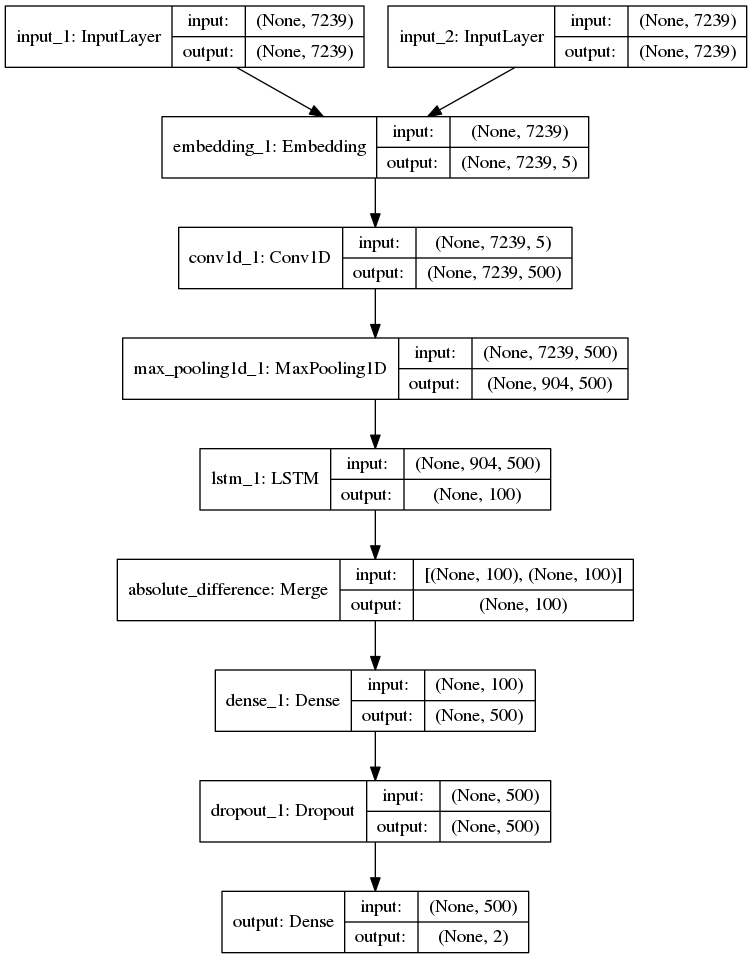
\includegraphics[width=\textwidth]{./pictures/experiments/network5.png}
    %\caption{Illustrate the structure of our fifth Siamese Neural Network.
        %Weights are shared by the embedding layers, the convolutional layer and
        %the LSTM layer. This Figure will be replaced by the new format when we
        %decide what that format is.}
    %\label{fig:network5}
%\end{figure}

%The network reached an accuracy of 0.89393 in epoch 18. The training and
%validation accuracies are shown in Figure \ref{fig:network_5_accuracies}. At the
%end of the training the network suddenly goes from about 90\% accuracy and back
%to 50\% accuracy. A reason for that happening could be that the optimizer
%overshot a target and therefore ended up with a worse result.

%\begin{figure}
    %\centering
    %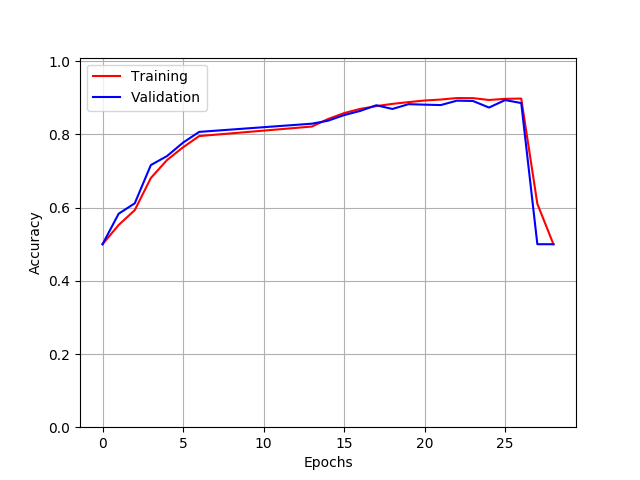
\includegraphics[width=0.5\textwidth]{./pictures/experiments/network_5_accuracies.png}
    %\caption{Shows the training and validation accuracies over the epochs of
        %training on the fifth iteration of our networks.}
    %\label{fig:network_5_accuracies}
%\end{figure}

%The students normally write their personal information in the beginning of
%assignments. Earlier we described that MaCom removed most of the names from
%the assignment. But they still contain information such as classes, dates and
%a different number of new line characters per student. We were suspicious
%that the networks still made use of some meta data from the texts so we tried
%training the network again but where we removed the 200 first characters from
%each text. Since most of the metadata are located in the beginning of the
%text we hoped that that would remove the problem. On this new dataset the
%best validation accuracy was obtained in epoch 3 with an accuracy of 0.53233.
%Clearly the network relied exclusively on the metadata in the beginning of
%the texts. We have shown the training and validation accuracies in Figure
%\ref{fig:network_5_accuracies_2}.

%\begin{figure}
    %\centering
    %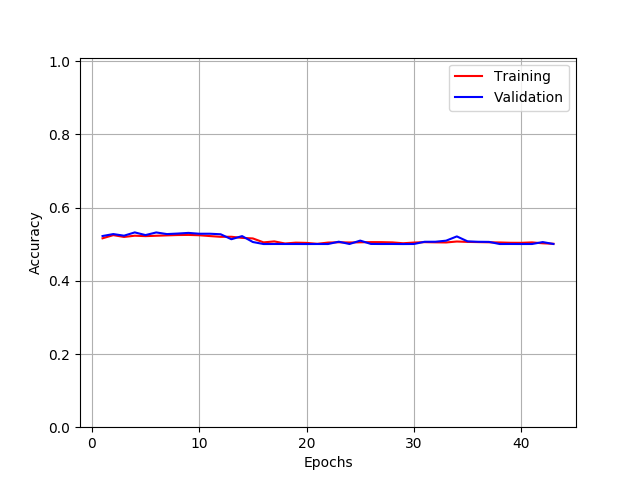
\includegraphics[width=0.5\textwidth]{./pictures/experiments/network_5_accuracies_2.png}
    %\caption{Shows the training and validation accuracies over the epochs of
        %training on the fifth iteration of our networks where we removed the 200
        %first characters.}
    %\label{fig:network_5_accuracies_2}
%\end{figure}


%\subsubsection{Siamese Neural Network - Iteration 6}
%\label{subsubsec:siamese_neuraon_network_iteration_6}

%In this iteration we trained our third network again but this time with the 200
%first characters removed like in Iteration 5. We wanted to see how much worse
%the network would perform now that we had hopefully removed some more personal
%information from what the network had available to look at. We have shown the
%training and validation accuracies in Figure \ref{fig:network_6_accuracies}. The
%best validation accuracy was obtained in epoch 57 with an accuracy of 0.74370.
%That means that we lost about 5\% accuracy by removing the first 200 characters.

%\begin{figure}
    %\centering
    %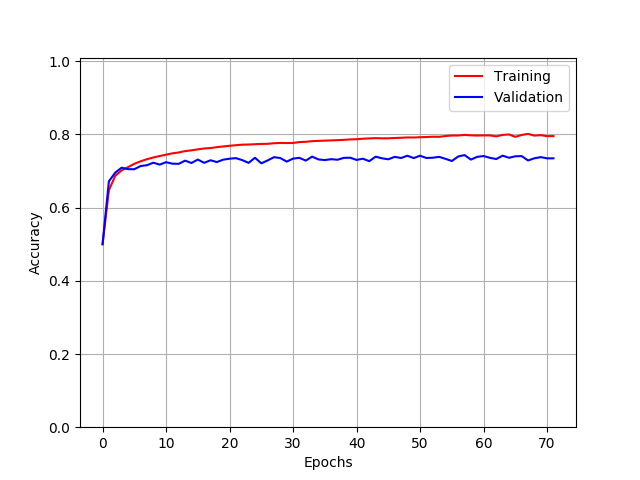
\includegraphics[width=0.5\textwidth]{./pictures/experiments/network_6_accuracies.png}
    %\caption{Shows the training and validation accuracies over the epochs of
        %training on the sixth iteration of our networks.}
    %\label{fig:network_6_accuracies}
%\end{figure}


%\subsubsection{Siamese Neural Network - Iteration 7}

%Since the overall performance and runtime of our network described in iterations
%5 did not perform very well, we chose a other route in terms of the \gls{RNN}'s.
%Using the approaches described in \cite{qian:2018} with some minor changes. A
%keras generated model can be seen in Figure \ref{fig:r_network6}.

%\begin{figure}
    %\centering
    %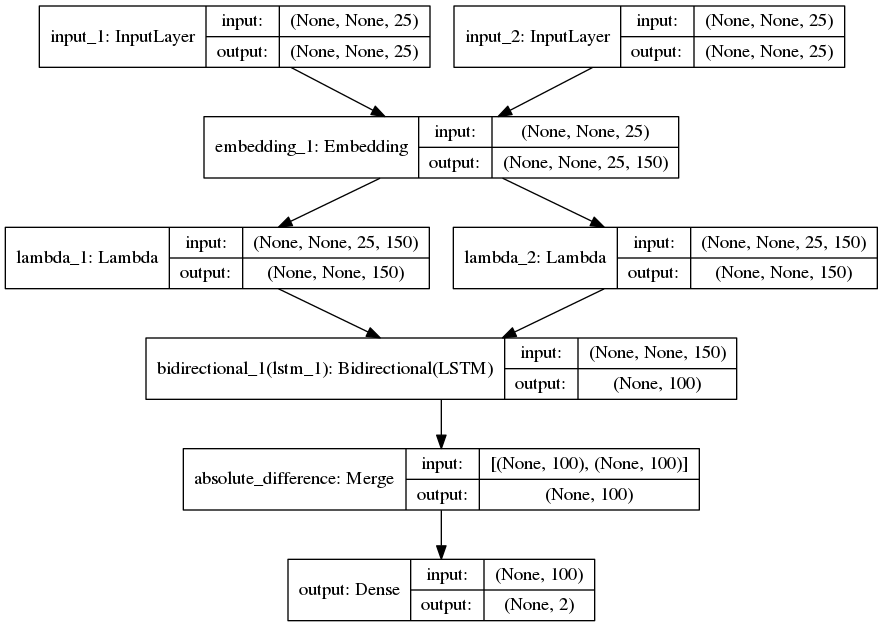
\includegraphics[width=0.5\textwidth]{./pictures/experiments/network6.png}
    %\caption{A keras generated model, showing the design of the \cite{qian:2018}
        %inspired network.}
    %\label{fig:r_network6}
%\end{figure}

%Contrary to previous networks we've produced, this network works on a higher
%linguistic level, by using words and sentences rather than characters. It does
%so by initially representing each text as a sequence of sequences. The outer
%sequence is a sentence and the inner sequence is the words of that sentence.
%We then proceed with representing each sentence as the sum of the embedded
%words in it. Each words is embedded to a vector of size 150, resulting in the
%summarized vector being the same size. Each of these summations are given to a
%bidirectional \gls{LSTM} layer, of 50 neurons. All this is done in a Siamese
%fashion so we have two branches of computation for each of the two texts given
%to the network, which are merged using the absolute difference. After this is
%done we simply feed this into a softmax dense layer to get the predictions.

%All sentences are padded and truncated to have length 25 and all texts in each
%batch are padded with 0 vectors to have the same length in sentences as the
%longest text in the batch. We use a bidirectional \gls{LSTM} to allow the
%network to use context from both sides of the current timestep.

%We have shown the training accuracy and validation accuracy in Figure
%\ref{fig:network_7_accuracies} (clearly we need to train some more epochs which
%should be running at the moment). The highest validation accuracy was obtained
%in epoch two with accuracy 0.92075.

%\begin{figure}
    %\centering
    %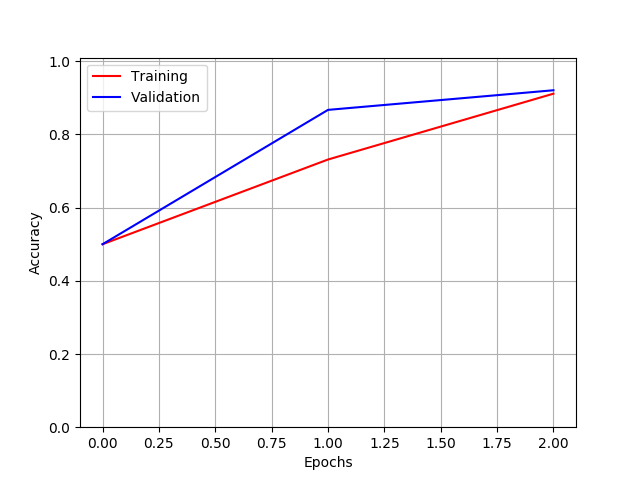
\includegraphics[width=0.5\textwidth]{./pictures/experiments/network_7_accuracies.png}
    %\caption{Shows the training and validation accuracies over the epochs of
        %training on the seventh iteration of our networks.}
    %\label{fig:network_7_accuracies}
%\end{figure}


%\subsubsection{Siamese Neural Network - Iteration 8}

%In this iteration we tried an extended version of the previous network. We used
%two bidirectional \gls{LSTM} layers on top of the word embeddings from before.
%Both of them returned sequences and we computed the final "features" by taking
%the average of the returned sequences giving us 50 numbers which indicated the
%author. We had huge problems with overfitting of the network on the training
%data authors. We have shown a graph of the training and validation accuracies
%in Figure \ref{fig:network_8_accuracies}.


%\subsubsection{Siamese Neural Network - Iteration 9}

%In this iteration we went back to using convolutional neural networks. Now we
%tried using both embedded words and embedded characters. We had a two
%convolutional layers for the characters, one looking at 8 characters and one
%looking at 4. For the words we had a convolutional layer looking at 8 words at a
%time. After the convolutional layer we had a max over time pooling layer for
%each of the filters and we combined the output for 2 texts with the absolute
%difference. We then had a densely connected network on top of that which learned
%from the features extracted. The dense network had 2 layers with 500 neurons in
%each. After that we had 30\% dropout and a softmax layer as usual.


\subsubsection{\glsdesc{rec-sent-NN}}
\label{subsubsec:rec_sent_nn}

After having attempted some convolutional approaches, as was just described,
we proceeded with some recurrent experiments as well. After having looked at
previous experiments made described in \cite{qian:2018}, which showed real
promise in terms of authorship attribution, we considered this a natural
extension of our convolutional approaches. Every \gls{RNN} experiment
was performed on the same data as the convolutional networks, and the
\textit{Embedding}, \textit{Feature Extraction}, \textit{Combining} and
\textit{Comparing} structure was used as for each of them too, and the best
model used can be seen depicted in figure [TODO].

\begin{description}

    \item[Embedding:] Test

\end{description}








 Like with the
convolutions, categorical loss, the Adam optimizer and a finishing 2 neuron
dense layer with a soft-max activation was used.

The first \gls{RNN}s made, was the first attempt at replicating the some of
the final networks described by \cite{qian:2018}. The network would still only
use 1 channel, the character channels, and have each of the two input texts
move through the network in a parallel fashion between layers sharing weights.
Instead of performing convolutions in the \textit{Feature Extraction} part of
the network, we used a \gls{GRU} layer with 200 units instead. Additionally
some comprehensive changed were made to both the \textit{Combining} and
\textit{Comparing} part of the network, which made use of the cosine distance
between the two texts, rather than the absolute difference between their
features, which is the basis of many of the networks we produced. This idea of
the cosine distance as the \textit{Comparing} part of the network, was attempted
in later iterations as well, but never yielded very good results compared to the
using of dense layers, which was the go to comparison approach from this point
forward.

In addition to the lack of accuracy yielded by a distance measure, this network
also revealed the gigantic computational requirements a \gls{RNN} needed,
having epoch training times of over 40 hours. Time we simply did not have. As
such the experiment from this point on focused mostly on increasing decreasing
computation time on an \gls{RNN} which made use of denser layers in the
\textit{Comparing} part of the network. This attempted decrease in computation
time took many forms. After some minor attempts relating to the number of units
in our recurrent layer, we concluded that the assailant was not the number of
units, but the amount of data used provided to the \textit{Feature Extraction}
part of the network. For that reason convolutional layers and max pooling layers
were included before the \gls{RNN} in the \textit{Feature Extraction} part of
the network. The purpose of this was to reduce the amount of data given to the
\gls{RNN} layers, with the potential additional up-side that the convolutions
would uncover something the \gls{RNN} could not, such as was done in several
of our previous convolutional networks. This largely reduced amount of data
expectedly decreased the amount of time needed for one epoch, from days down to
hours. The accuracies of these convolution, \gls{RNN} hybrids were however not
very good, all lying around the 50\% accuracy mark, which of course for a 50/50
data set, is the worst accuracy possible. Even switching out the \gls{GRU} with
and \gls{LSTM} layer, did not do the networks any favors.

At this point we deem \gls{RNN}s feasible at the current linguistic level.
This we move the level up, creating networks that based themselves on the
sentence level of the provided texts. The best performing \gls{RNN}, among
other changes, made use of this sentence level approach. The overall design of
this network can be seen in Figure [TODO]. Each text provided to the network is
represented as a sequence of sequences. Each element in the outer sequence is
considered a sentence, which is represented by a sequence of 25 words from the
provided text. As such, the text is represented a sequence its the words from
the texts, split into chunks of 25 words piece. It in this state, we provide the
text to the first part of the network, the \textit{Embedding}. At this stage we
parse all the words of each sentence through an embedding layer. In the earlier
iterations of both the \gls{RNN} and the convolutions, these were trained along
with the entire network. But as computation time/accuracy become increasingly
a concern, we opted for pre-trained embeddings \cite{bojanowski2016}. These
pre-trained embeddings mapped each word into a vector of length 300. As expected
this did in fact improve on the computation time, and it did so without harming
the validation accuracy. With each word embedded, we took the average of each 25
word sequence which now serves at the representation of the sentence the words
were assigned before. Now having each sentence represented, we proceed to the
next part, \textit{Feature Extraction}. For our best \gls{RNN}s, this process
consisted of using simply using a bidirectional \gls{LSTM} layer. Like in the
convolutions the absolute difference between these two feature-sets would be
computes, and in this case be provided directly to the dense output layer. This
bidirectional layer, consisted of 50 neurons, thus ending up with a total of
100 output. The \gls{LSTM} layer makes use of the default parameters as well.
This being using the Tanh activation function, seen in Equation \eqref{eq:tanh},
when finished, and the Hard Sigmoid activation function, seen in Equation
\eqref{eq:h_sig}, at each recurrent step.

\begin{equation}\label{eq:tanh}
h(x) = \tanh(x) = \frac{(e^x - e^{-x})}{(e^x + e^{-x})}
\end{equation}

\begin{equation}\label{eq:h_sig}
h(x) = \max(0, \min(1, x \cdot 0.2 + 0.5))
\end{equation}

The Adam optimizer also made use of the default parameters, $\eta = 0.001$,
$\gamma_1 = 0.9$ and $\gamma_2=0.999$. and a decay of 0. As the loss function we
used the categorical cross-entropy function.

Using this sentence level \gls{RNN} yielded surprisingly great result initially.
However, after having applied these results to the prediction system, a big
flaw became apparent. During training the validation accuracy of network
extremely good getting results in the 90\% range, the 50/50 data set it was
given. But when given to the prediction system, the results were horrific. In
our initial split of the data, authors would be present in both the training
data applied to the network, and the validation data used after each epoch to
determine the unbiased performance of the network. This was the cause of the
problem. The goal of the networks we produced for this paper, was to generalize
of all students. The network did however learn each specific student very
well, and for that reason the presence of the student in was trained on in the
validation set, made predictions very easy, resulting in the high accuracy.
After fixing this data sample creation problem, the results aligned with the
ones produced by the prediction system. These results can be seen in figure
\ref{fig:network_8_accuracies}.

\begin{figure}
    \centering
    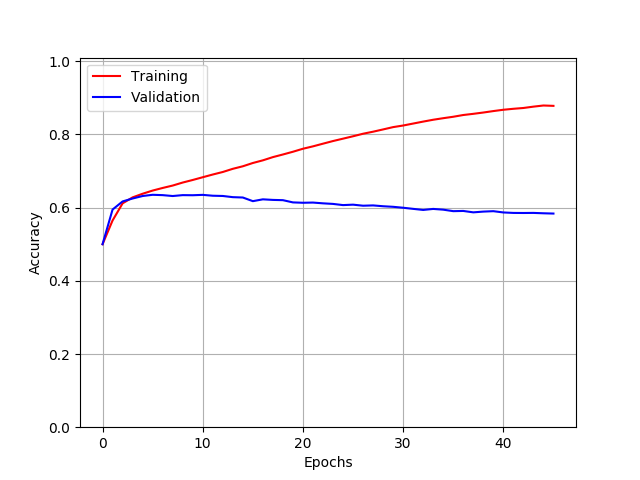
\includegraphics[width=0.5\textwidth]{./pictures/experiments/network_8_accuracies.png}
    \caption{Shows the training and validation accuracies over the epochs of
        training on the eighth iteration of our networks.}
    \label{fig:network_8_accuracies}
\end{figure}


\subsection{Prediction System}

Our prediction system has several hyperparameters we have to choose to get
the best results. We recall that MaCom wanted a system that had an accusation
error of less than 10\%. We can use the threshold parameter $\theta$ in the
prediction system to control how many people we accuse. The best parameters
for the prediction system is those parameters that gives the highest accuracy
subject to the constraint that the accusation error should be less than 10\%.
To tune the parameters we use a validation dataset $V$ consisting of a set of
tuples $(\alpha, t_u)$ where $\alpha$ is a candidate author and $t_u$ is a text
of unknown authorship. None of the authors in $V$ has been seen by the networks
during training and none of the texts $t_u$ has been seen by the networks during
training. The parameters that maximize the accuracy subject to the bounded
accusation error is the same as the parameters that minimize the error rate
subject to the bounded accusation error. That optimization problem is,

\begin{equation}
    \label{eq:prediction_system_minimization}
    \begin{aligned}
        & \underset{\theta, w}{\text{minimize}}
        & & \sum_{(\alpha, t_u) \in V} \left|
            P(f, w, T_\alpha \setminus \{t_u\}, t_u, \theta) -
            \mathbbm{1}_{T_\alpha}(t_u)
        \right| \\
        & \text{subject to}
        & & \frac{\sum_{(\alpha, t_u) \in V} \mathbbm{1}_{T_\alpha}(t_u) \cdot
            \left(1 - P(f, w, T_\alpha \setminus \{t_u\}, t_u, \theta)\right)}
{\sum_{(\alpha, t_u) \in V} (1 - P(f, w, T_\alpha \setminus \{t_u\}, t_u, \theta)} <
            \frac{1}{10}
    \end{aligned}
\end{equation}

In the optimization problem we fix the network $f$ we validate. The expression
we minimize is the number of errors made in prediction over the validation set
$V$. Consider a problem $(\alpha, t_u) \in V$ where $t_u \in T_\alpha$. Then we
know that $\mathbbm{1}_{T_\alpha}(t_u) = 1$ from the definition of the indicator
function then if the prediction system returns the correct result 1 we have,

\begin{equation}
    e = \left|
        P(f, w, T_\alpha \setminus \{t_u\}, t_u, \theta) -
        \mathbbm{1}_{T_\alpha}(t_u)
    \right| = |1 - 1| = 0,
\end{equation}

and if the prediction system returns the incorrect result 0 we have,

\begin{equation}
    e = \left|
        P(f, w, T_\alpha \setminus \{t_u\}, t_u, \theta) -
        \mathbbm{1}_{T_\alpha}(t_u)
    \right| = |0 - 1| = 1.
\end{equation}

Similarly for a problem $(\alpha, t_u) \in V$ where $t_u \notin T_\alpha$ we
know that $\mathbbm{1}_{T_\alpha}(t_u) = 0$ from the definition of the indicator
function. Then if the prediction system returns the correct result 0 we have,

\begin{equation}
    e = \left|
        P(f, w, T_\alpha \setminus \{t_u\}, t_u, \theta) -
        \mathbbm{1}_{T_\alpha}(t_u)
    \right| = |0 - 0| = 0, \end{equation}

and if the prediction system returns the incorrect result 1 we have,

\begin{equation}
    e = \left|
        P(f, w, T_\alpha \setminus \{t_u\}, t_u, \theta) -
        \mathbbm{1}_{T_\alpha}(t_u)
    \right| = |1 - 0| = 1.
\end{equation}

That is the expression we minimize is 0 whenever there is no error and 1
whenever there is an error. So we minimize the number of errors we make. The
subject to expression makes sure that the fraction of false accusations we make
is less than $10\%$ of the accusations we make. The expression should be read
as,

\begin{equation}
    \frac{\textit{false accusations}}{\textit{total accusations}} < \frac{1}{10}
\end{equation}

Consider the numerator of the fraction on the left hand side,

\begin{equation}
    \textit{false accusations} = \sum_{(\alpha, t_u) \in V}
    \mathbbm{1}_{T_\alpha}(t_u) \cdot
    \left(1 - P(f, w, T_\alpha \setminus \{t_u\}, t_u, \theta)\right).
\end{equation}

For a $(\alpha, t_u) \in V$ where $t_u \in T_\alpha$ we have that
$\mathbbm{1}_{T_\alpha}(t_u) = 1$ then if $P$ is correct it returns 1 and we
get,

\begin{equation}
    \mathbbm{1}_{T_\alpha}(t_u) \cdot
    \left(1 - P(f, w, T_\alpha \setminus \{t_u\}, t_u, \theta)\right) =
    1 \cdot (1 - 1) = 0,
\end{equation}

and if $P$ is incorrect and returns 0 we have,

\begin{equation}
    \mathbbm{1}_{T_\alpha}(t_u) \cdot
    \left(1 - P(f, w, T_\alpha \setminus \{t_u\}, t_u, \theta)\right) =
    1 \cdot (1 - 0) = 1.
\end{equation}

Similarly for a $(\alpha, t_u) \in V$ where $t_u \in T_\alpha$ we have that
$\mathbbm{1}_{T_\alpha}(t_u) = 0$ and therefore the expression is always
0. Therefore the expression is 1 whenever we have a false accusation and 0
otherwise. The right hand side of the inequality simply counts the number of
accusations by inverting the output of $P$ and divides that by 10. So the
condition makes sure that only 10\% of the accusations we make are false
accusations.

We find the optimal parameters by doing a binary search for
the threshold $\theta$ that solves the minimization problem
\eqref{eq:prediction_system_minimization} for each weight function. We start
the search with a lower threshold of 0.0 and an upper threshold of 1.0. Then we
continue the search for $\theta$ until we have converged on a fixed point. The
thresholds and weights we report as the optimum for the networks are based on
the output of this binary search.

We have run our prediction system on several of the networks we trained as
part of our experiments. For each of the networks we present several graphs
showing their performance for different weights and thresholds and we report
the best configuration for that network. The dataset we use to tune $\theta$
and the weight function $w$ are F. The set consists of 2000 previously unseen
authors. From them we generate two problems for each author meaning that we
end up with 4000 different problems. For each of the authors we generate a
positive sample by taking the newest text as the unknown text and a negative
sample by choosing a random text from some other author in the set. That is
we have a 0.5 split between positive and negative samples. We also tried our
prediction system on another validation set. In the real world it has been
estimated that 4\% of turn ins for the \gls{SRP} are written by "ghost writers"
\footnote{https://politiken.dk/indland/uddannelse/art5603163/Gymnasieelever-\%C2
\% BBSnyderi-beviser-hvor-vanvittig-betydningsfuld-SRP-er-blevet\%C2\%AB}. We
therefore also wanted to find the $\theta$ and $w$ for a validation set with
only 4\% negative samples instead of 50\% negative samples. We generated 2000
positive samples as before and then for each sample we added a negative sample
with a 4\% chance.


\subsubsection{Convolutional Siamese Neural Network 1}

The first network we tuned hyperparameters for were the network presented
in Figure TODO. The network used only convolutions on the character level
to extract features and used a dense network to decide whether or not
the texts were written by the same author. We have shown the accuracy
and accusation error for the dataset containing 50\% negatives in Figure
\ref{fig:prediction_system_results_1} and for the dataset containing 4\%
negatives in Figure \ref{fig:prediction_system_results_2}.

\begin{figure}
    \centering
    \textbf{Prediction System Results for 0.5 Split}\par\medskip
    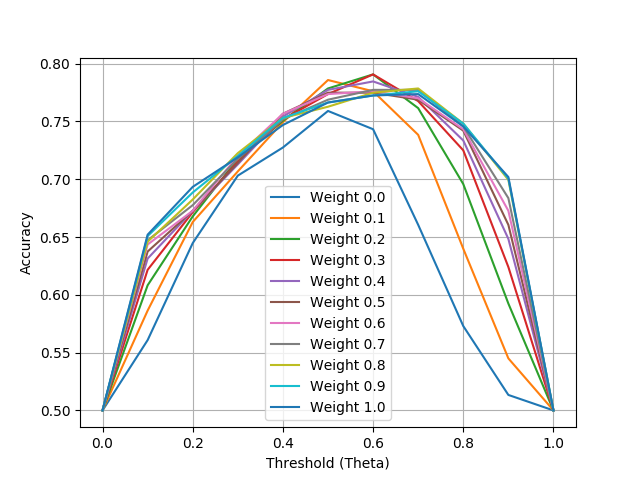
\includegraphics[width=0.8\textwidth]{./pictures/experiments/network3_prediction_system_accuracies.png}
    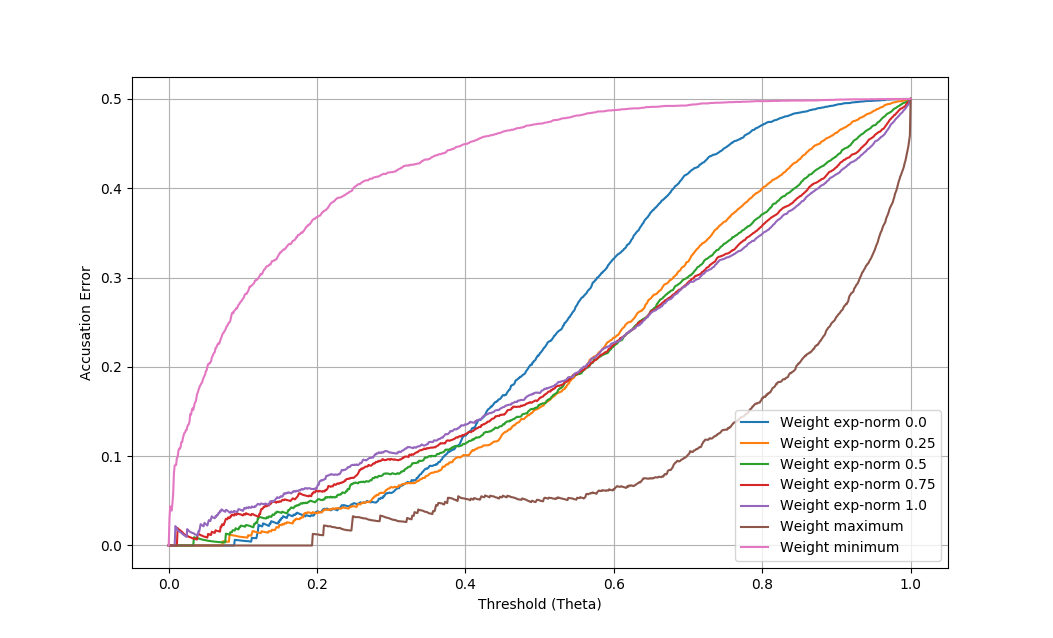
\includegraphics[width=0.8\textwidth]{./pictures/experiments/network3_prediction_system_accusation_error.png}
    \caption{Results of running the prediction system with the network described
        in Section \ref{subsubsec:convolutional_siamese_neural_networks} on a
        validation dataset with 50\% positive samples and 50\% negative samples.
        In the upper graph we show the accuracies obtained as a function of
        $\theta$ for different weights $w$. At the bottom we have shown the
        accusation error as a function $\theta$ again with one line for each
        weight. We can see that as the threshold increases and we accuse more
        people of cheating the accusation error rises.}
    \label{fig:prediction_system_results_1}
\end{figure}

\begin{figure}
    \centering
    \textbf{Prediction System Results for 0.04 Split}\par\medskip
    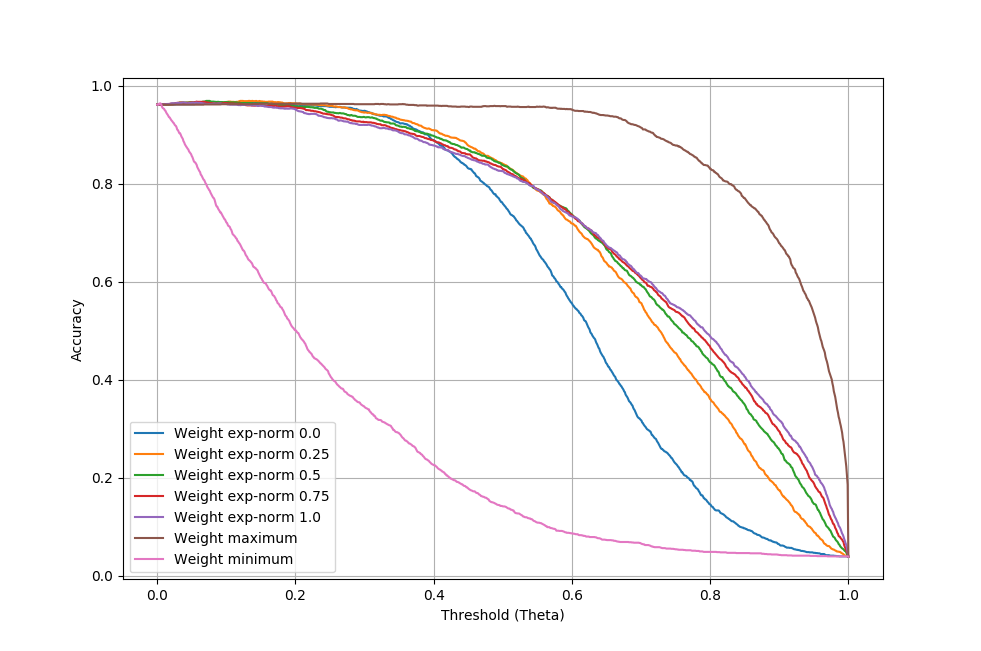
\includegraphics[width=0.8\textwidth]{./pictures/experiments/network3_prediction_system_accuracies_4_percent.png}
    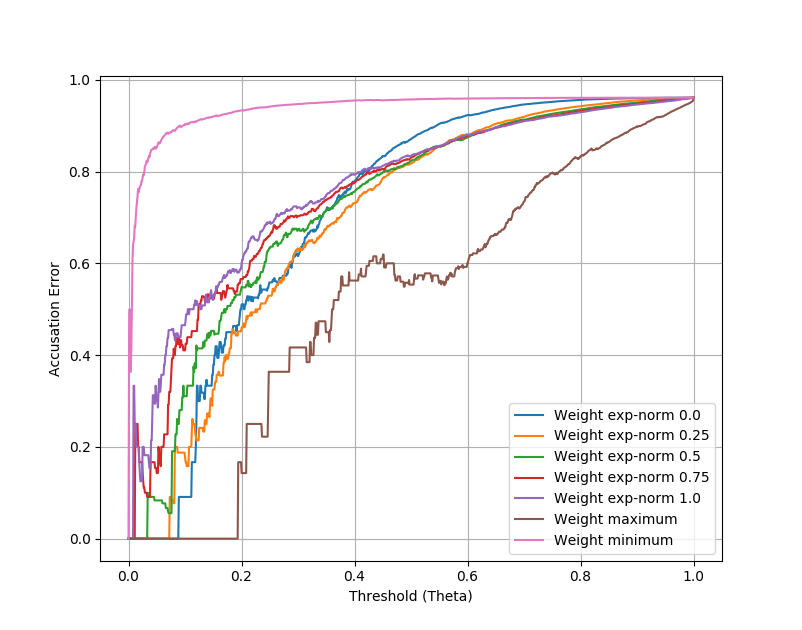
\includegraphics[width=0.8\textwidth]{./pictures/experiments/network3_prediction_system_accusation_error_4_percent.png}
    \caption{Results of running the prediction system with the network described
        in Section \ref{subsubsec:convolutional_siamese_neural_networks} on a
        validation dataset with 96\% positive samples and 4\% negative samples.
        In the upper graph we show the accuracies obtained as a function of
        $\theta$ for different weights $w$. At the bottom we have shown the
        accusation error as a function $\theta$ again with one line for each
        weight. We can see that as the threshold increases and we accuse more
        people of cheating the accusation error rises.}
    \label{fig:prediction_system_results_2}
\end{figure}

The best configuration for the 0.5 split were using the Exponential Norm Weight
function with $\lambda = 0.25$ and using the threshold $\theta = 0.395398$.
That configuration obtained an accusation error of 9.9761\% and an accuracy of
83.5168 \%. The configuration had 1507 \gls{TN}s, 1832 \gls{TP}s, 167 \gls{FN}s
and 492 \gls{FP}s. The best configuration for the 0.04 split were using the
Exponential Norm Weight function with $\lambda = 0.5$ and using the threshold
$\theta = 0.076101$. That configuration obtained an accusation error of 5.5556
\% and an accuracy of 96.8750 \%. The configuration had 17 \gls{TN}s, 1998
\gls{TP}s, 1 \gls{FN}s and 64 \gls{FP}s.


\subsubsection{Convolutional Siamese Neural Network 2}

The second network we tuned hyperparameters for were the network presented
in Figure TODO. The network used convolutions on the character level and
word level to extract features and used a dense network to decide whether or
not the texts were written by the same author. We have shown the accuracy
and accusation error for the dataset containing 50\% negatives in Figure
\ref{fig:prediction_system_results_3} and for the dataset containing 4\%
negatives in Figure \ref{fig:prediction_system_results_4}.

\begin{figure}
    \centering
    \textbf{Prediction System Results for 0.5 Split}\par\medskip
    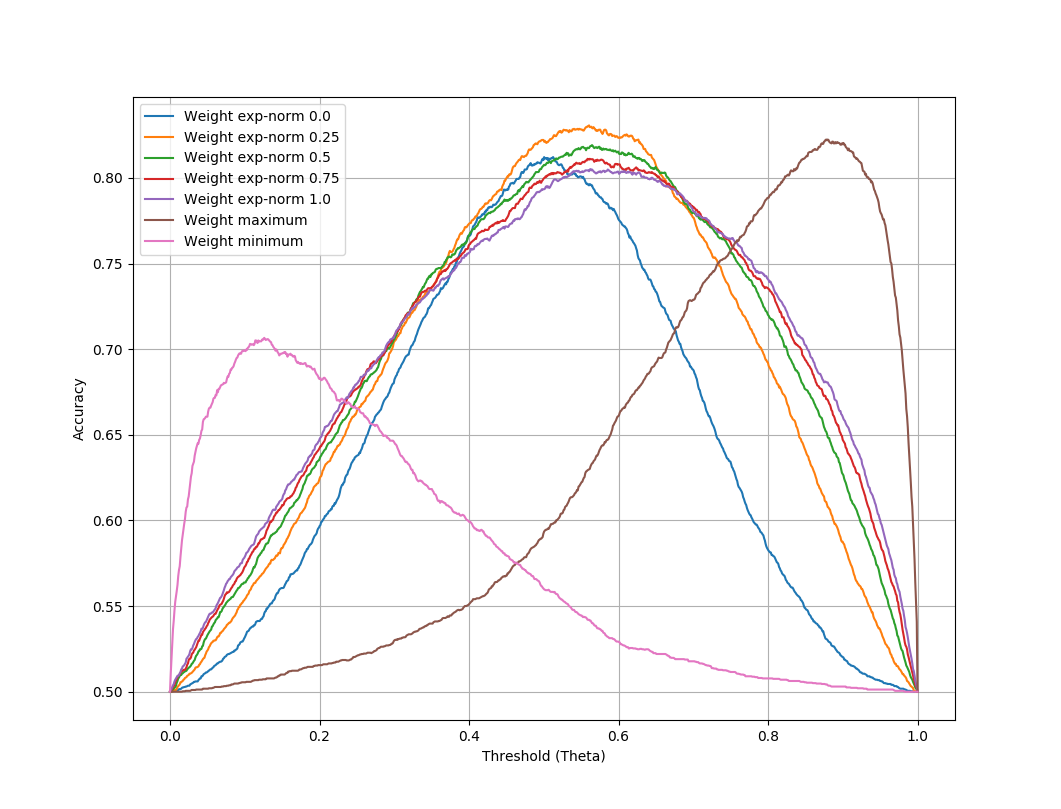
\includegraphics[width=0.8\textwidth]{./pictures/experiments/network6_prediction_system_accuracies.png}
    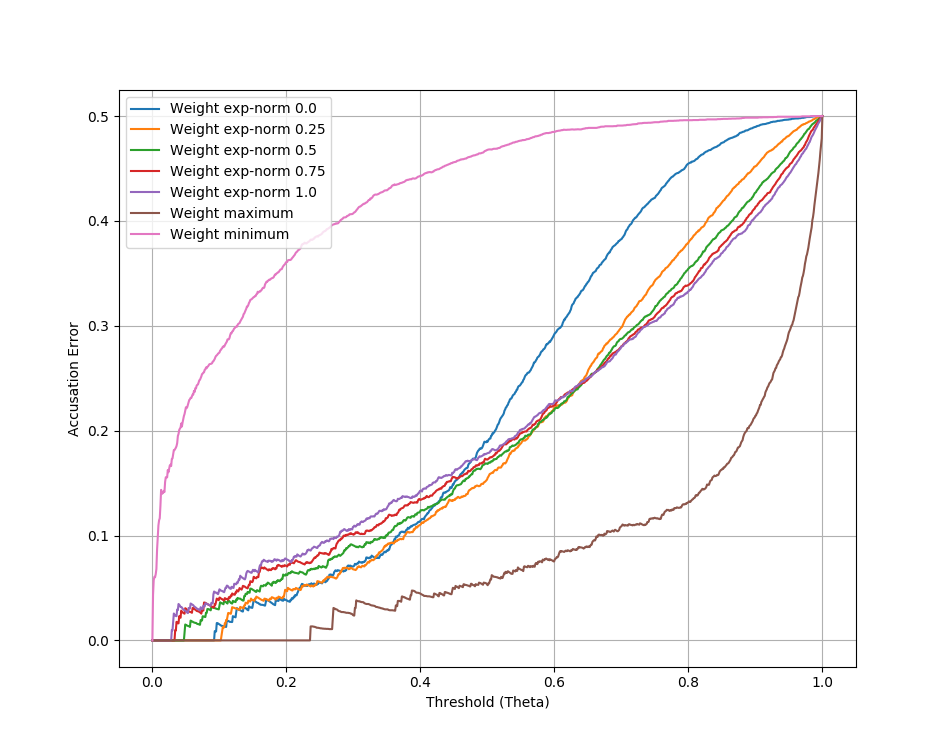
\includegraphics[width=0.8\textwidth]{./pictures/experiments/network6_prediction_system_accusation_error.png}
    \caption{Results of running the prediction system with the network described
        in Section \ref{subsubsec:convolutional_siamese_neural_networks} on a
        validation dataset with 50\% positive samples and 50\% negative samples.
        In the upper graph we show the accuracies obtained as a function of
        $\theta$ for different weights $w$. At the bottom we have shown the
        accusation error as a function $\theta$ again with one line for each
        weight. We can see that as the threshold increases and we accuse more
        people of cheating the accusation error rises.}
    \label{fig:prediction_system_results_3}
\end{figure}

\begin{figure}
    \centering
    \textbf{Prediction System Results for 0.04 Split}\par\medskip
    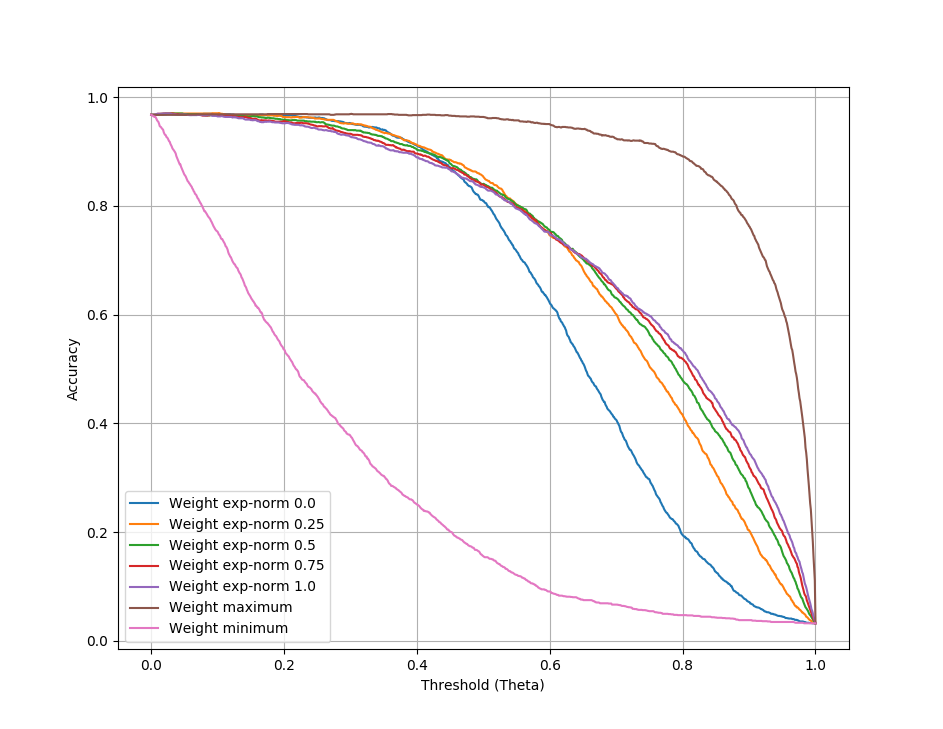
\includegraphics[width=0.8\textwidth]{./pictures/experiments/network6_prediction_system_accuracies_4_percent.png}
    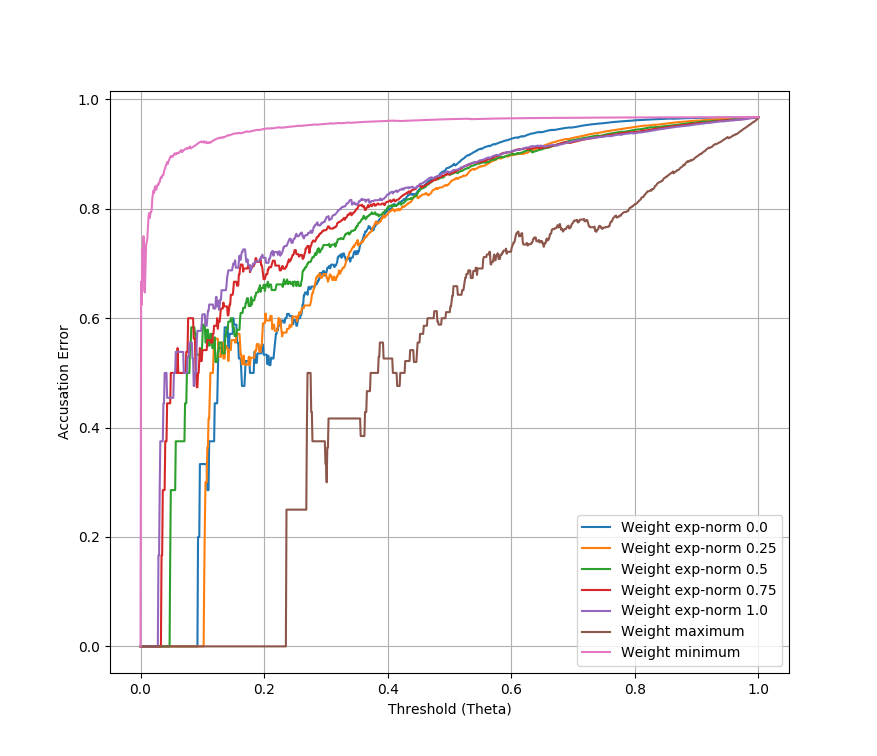
\includegraphics[width=0.8\textwidth]{./pictures/experiments/network6_prediction_system_accusation_error_4_percent.png}
    \caption{Results of running the prediction system with the network described
        in Section \ref{subsubsec:convolutional_siamese_neural_networks} on a
        validation dataset with 96\% positive samples and 4\% negative samples.
        In the upper graph we show the accuracies obtained as a function of
        $\theta$ for different weights $w$. At the bottom we have shown the
        accusation error as a function $\theta$ again with one line for each
        weight. We can see that as the threshold increases and we accuse more
        people of cheating the accusation error rises.}
    \label{fig:prediction_system_results_4}
\end{figure}

The best configuration for the 0.5 split were using the Exponential Norm Weight
function with $\lambda = 0.25$ and using the threshold $\theta = 0.376832$.
That configuration obtained an accusation error of 9.9766\% and an accuracy of
75.6878 \%. The configuration had 1155 \gls{TN}s, 1871 \gls{TP}s, 128 \gls{FN}s
and 844 \gls{FP}s. The best configuration for the 0.04 split were using the
Maximum Weight function and using the threshold $\theta = 0.235470$. That
configuration obtained an accusation error of 0 \% and an accuracy of 96.9022
\%. The configuration had 3 \gls{TN}s, 1999 \gls{TP}s, 0 \gls{FN}s and 64
\gls{FP}s.
